\documentclass[twoside]{book}

% Packages required by doxygen
\usepackage{fixltx2e}
\usepackage{calc}
\usepackage{doxygen}
\usepackage[export]{adjustbox} % also loads graphicx
\usepackage{graphicx}
\usepackage[utf8]{inputenc}
\usepackage{makeidx}
\usepackage{multicol}
\usepackage{multirow}
\PassOptionsToPackage{warn}{textcomp}
\usepackage{textcomp}
\usepackage[nointegrals]{wasysym}
\usepackage[table]{xcolor}

% Font selection
\usepackage[T1]{fontenc}
\usepackage[scaled=.90]{helvet}
\usepackage{courier}
\usepackage{amssymb}
\usepackage{sectsty}
\renewcommand{\familydefault}{\sfdefault}
\allsectionsfont{%
  \fontseries{bc}\selectfont%
  \color{darkgray}%
}
\renewcommand{\DoxyLabelFont}{%
  \fontseries{bc}\selectfont%
  \color{darkgray}%
}
\newcommand{\+}{\discretionary{\mbox{\scriptsize$\hookleftarrow$}}{}{}}

% Page & text layout
\usepackage{geometry}
\geometry{%
  a4paper,%
  top=2.5cm,%
  bottom=2.5cm,%
  left=2.5cm,%
  right=2.5cm%
}
\tolerance=750
\hfuzz=15pt
\hbadness=750
\setlength{\emergencystretch}{15pt}
\setlength{\parindent}{0cm}
\setlength{\parskip}{3ex plus 2ex minus 2ex}
\makeatletter
\renewcommand{\paragraph}{%
  \@startsection{paragraph}{4}{0ex}{-1.0ex}{1.0ex}{%
    \normalfont\normalsize\bfseries\SS@parafont%
  }%
}
\renewcommand{\subparagraph}{%
  \@startsection{subparagraph}{5}{0ex}{-1.0ex}{1.0ex}{%
    \normalfont\normalsize\bfseries\SS@subparafont%
  }%
}
\makeatother

% Headers & footers
\usepackage{fancyhdr}
\pagestyle{fancyplain}
\fancyhead[LE]{\fancyplain{}{\bfseries\thepage}}
\fancyhead[CE]{\fancyplain{}{}}
\fancyhead[RE]{\fancyplain{}{\bfseries\leftmark}}
\fancyhead[LO]{\fancyplain{}{\bfseries\rightmark}}
\fancyhead[CO]{\fancyplain{}{}}
\fancyhead[RO]{\fancyplain{}{\bfseries\thepage}}
\fancyfoot[LE]{\fancyplain{}{}}
\fancyfoot[CE]{\fancyplain{}{}}
\fancyfoot[RE]{\fancyplain{}{\bfseries\scriptsize Generated by Doxygen }}
\fancyfoot[LO]{\fancyplain{}{\bfseries\scriptsize Generated by Doxygen }}
\fancyfoot[CO]{\fancyplain{}{}}
\fancyfoot[RO]{\fancyplain{}{}}
\renewcommand{\footrulewidth}{0.4pt}
\renewcommand{\chaptermark}[1]{%
  \markboth{#1}{}%
}
\renewcommand{\sectionmark}[1]{%
  \markright{\thesection\ #1}%
}

% Indices & bibliography
\usepackage{natbib}
\usepackage[titles]{tocloft}
\setcounter{tocdepth}{3}
\setcounter{secnumdepth}{5}
\makeindex

% Hyperlinks (required, but should be loaded last)
\usepackage{ifpdf}
\ifpdf
  \usepackage[pdftex,pagebackref=true]{hyperref}
\else
  \usepackage[ps2pdf,pagebackref=true]{hyperref}
\fi
\hypersetup{%
  colorlinks=true,%
  linkcolor=blue,%
  citecolor=blue,%
  unicode%
}

% Custom commands
\newcommand{\clearemptydoublepage}{%
  \newpage{\pagestyle{empty}\cleardoublepage}%
}

\usepackage{caption}
\captionsetup{labelsep=space,justification=centering,font={bf},singlelinecheck=off,skip=4pt,position=top}

%===== C O N T E N T S =====

\begin{document}

% Titlepage & ToC
\hypersetup{pageanchor=false,
             bookmarksnumbered=true,
             pdfencoding=unicode
            }
\pagenumbering{alph}
\begin{titlepage}
\vspace*{7cm}
\begin{center}%
{\Large Statistiche }\\
\vspace*{1cm}
{\large Generated by Doxygen 1.8.14}\\
\end{center}
\end{titlepage}
\clearemptydoublepage
\pagenumbering{roman}
\tableofcontents
\clearemptydoublepage
\pagenumbering{arabic}
\hypersetup{pageanchor=true}

%--- Begin generated contents ---
\chapter{Namespace Index}
\section{Packages}
Here are the packages with brief descriptions (if available)\+:\begin{DoxyCompactList}
\item\contentsline{section}{\mbox{\hyperlink{namespacemain}{main}} }{\pageref{namespacemain}}{}
\end{DoxyCompactList}

\chapter{Hierarchical Index}
\section{Class Hierarchy}
This inheritance list is sorted roughly, but not completely, alphabetically\+:\begin{DoxyCompactList}
\item \contentsline{section}{Main}{\pageref{classmain_1_1_main}}{}
\item \contentsline{section}{Shared\+Data}{\pageref{classmain_1_1_shared_data}}{}
\item Thread\begin{DoxyCompactList}
\item \contentsline{section}{Th\+Cerca}{\pageref{classmain_1_1_th_cerca}}{}
\item \contentsline{section}{Th\+Gen}{\pageref{classmain_1_1_th_gen}}{}
\item \contentsline{section}{Th\+Vis}{\pageref{classmain_1_1_th_vis}}{}
\end{DoxyCompactList}
\end{DoxyCompactList}

\chapter{Class Index}
\section{Class List}
Here are the classes, structs, unions and interfaces with brief descriptions\+:\begin{DoxyCompactList}
\item\contentsline{section}{\mbox{\hyperlink{classmain_1_1_main}{Main}} }{\pageref{classmain_1_1_main}}{}
\item\contentsline{section}{\mbox{\hyperlink{classmain_1_1_shared_data}{Shared\+Data}} }{\pageref{classmain_1_1_shared_data}}{}
\item\contentsline{section}{\mbox{\hyperlink{classmain_1_1_th_cerca}{Th\+Cerca}} }{\pageref{classmain_1_1_th_cerca}}{}
\item\contentsline{section}{\mbox{\hyperlink{classmain_1_1_th_gen}{Th\+Gen}} }{\pageref{classmain_1_1_th_gen}}{}
\item\contentsline{section}{\mbox{\hyperlink{classmain_1_1_th_vis}{Th\+Vis}} }{\pageref{classmain_1_1_th_vis}}{}
\end{DoxyCompactList}

\chapter{File Index}
\section{File List}
Here is a list of all files with brief descriptions\+:\begin{DoxyCompactList}
\item\contentsline{section}{Statistiche/src/main/\mbox{\hyperlink{_main_8java}{Main.\+java}} }{\pageref{_main_8java}}{}
\item\contentsline{section}{Statistiche/src/main/\mbox{\hyperlink{_shared_data_8java}{Shared\+Data.\+java}} }{\pageref{_shared_data_8java}}{}
\item\contentsline{section}{Statistiche/src/main/\mbox{\hyperlink{_th_cerca_8java}{Th\+Cerca.\+java}} }{\pageref{_th_cerca_8java}}{}
\item\contentsline{section}{Statistiche/src/main/\mbox{\hyperlink{_th_gen_8java}{Th\+Gen.\+java}} }{\pageref{_th_gen_8java}}{}
\item\contentsline{section}{Statistiche/src/main/\mbox{\hyperlink{_th_vis_8java}{Th\+Vis.\+java}} }{\pageref{_th_vis_8java}}{}
\end{DoxyCompactList}

\chapter{Namespace Documentation}
\hypertarget{namespacemain}{}\section{Package main}
\label{namespacemain}\index{main@{main}}
\subsection*{Classes}
\begin{DoxyCompactItemize}
\item 
class \mbox{\hyperlink{classmain_1_1_main}{Main}}
\item 
class \mbox{\hyperlink{classmain_1_1_shared_data}{Shared\+Data}}
\item 
class \mbox{\hyperlink{classmain_1_1_th_cerca}{Th\+Cerca}}
\item 
class \mbox{\hyperlink{classmain_1_1_th_gen}{Th\+Gen}}
\item 
class \mbox{\hyperlink{classmain_1_1_th_vis}{Th\+Vis}}
\end{DoxyCompactItemize}

\chapter{Class Documentation}
\hypertarget{classmain_1_1_main}{}\section{Main Class Reference}
\label{classmain_1_1_main}\index{Main@{Main}}


Collaboration diagram for Main\+:
\nopagebreak
\begin{figure}[H]
\begin{center}
\leavevmode
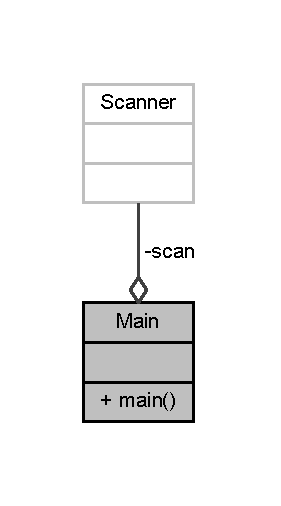
\includegraphics[width=135pt]{classmain_1_1_main__coll__graph}
\end{center}
\end{figure}
\subsection*{Static Public Member Functions}
\begin{DoxyCompactItemize}
\item 
static void \mbox{\hyperlink{classmain_1_1_main_a8b260eecbaabcef8473fd87ada040682}{main}} (String\mbox{[}$\,$\mbox{]} args)
\end{DoxyCompactItemize}
\subsection*{Static Private Attributes}
\begin{DoxyCompactItemize}
\item 
static final Scanner \mbox{\hyperlink{classmain_1_1_main_ad2b26d92ead66c3a1c4e4d4d77394aba}{scan}} = new Scanner(System.\+in)
\end{DoxyCompactItemize}


\subsection{Detailed Description}
\begin{DoxyAuthor}{Author}
mantica\+\_\+luca 
\end{DoxyAuthor}


Definition at line 15 of file Main.\+java.



\subsection{Member Function Documentation}
\mbox{\Hypertarget{classmain_1_1_main_a8b260eecbaabcef8473fd87ada040682}\label{classmain_1_1_main_a8b260eecbaabcef8473fd87ada040682}} 
\index{main\+::\+Main@{main\+::\+Main}!main@{main}}
\index{main@{main}!main\+::\+Main@{main\+::\+Main}}
\subsubsection{\texorpdfstring{main()}{main()}}
{\footnotesize\ttfamily static void main (\begin{DoxyParamCaption}\item[{String \mbox{[}$\,$\mbox{]}}]{args }\end{DoxyParamCaption})\hspace{0.3cm}{\ttfamily [static]}}



Definition at line 19 of file Main.\+java.

Here is the call graph for this function\+:
\nopagebreak
\begin{figure}[H]
\begin{center}
\leavevmode
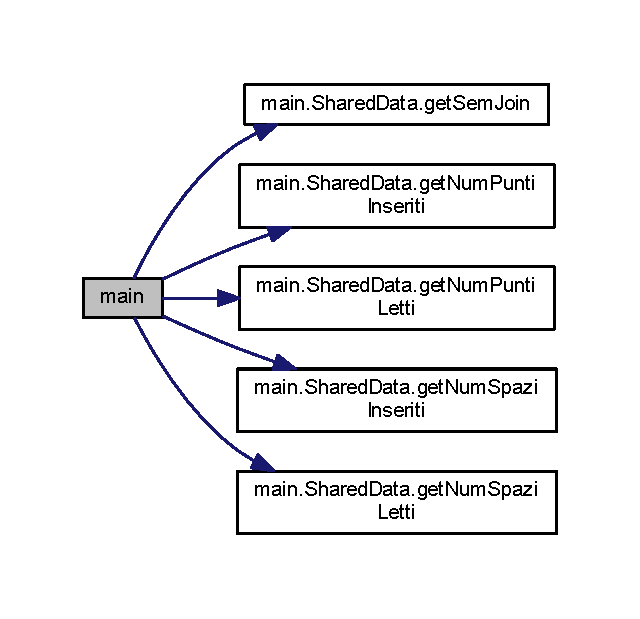
\includegraphics[width=307pt]{classmain_1_1_main_a8b260eecbaabcef8473fd87ada040682_cgraph}
\end{center}
\end{figure}


\subsection{Member Data Documentation}
\mbox{\Hypertarget{classmain_1_1_main_ad2b26d92ead66c3a1c4e4d4d77394aba}\label{classmain_1_1_main_ad2b26d92ead66c3a1c4e4d4d77394aba}} 
\index{main\+::\+Main@{main\+::\+Main}!scan@{scan}}
\index{scan@{scan}!main\+::\+Main@{main\+::\+Main}}
\subsubsection{\texorpdfstring{scan}{scan}}
{\footnotesize\ttfamily final Scanner scan = new Scanner(System.\+in)\hspace{0.3cm}{\ttfamily [static]}, {\ttfamily [private]}}



Definition at line 17 of file Main.\+java.



The documentation for this class was generated from the following file\+:\begin{DoxyCompactItemize}
\item 
Statistiche/src/main/\mbox{\hyperlink{_main_8java}{Main.\+java}}\end{DoxyCompactItemize}

\hypertarget{classmain_1_1_shared_data}{}\section{Shared\+Data Class Reference}
\label{classmain_1_1_shared_data}\index{Shared\+Data@{Shared\+Data}}


Collaboration diagram for Shared\+Data\+:
\nopagebreak
\begin{figure}[H]
\begin{center}
\leavevmode
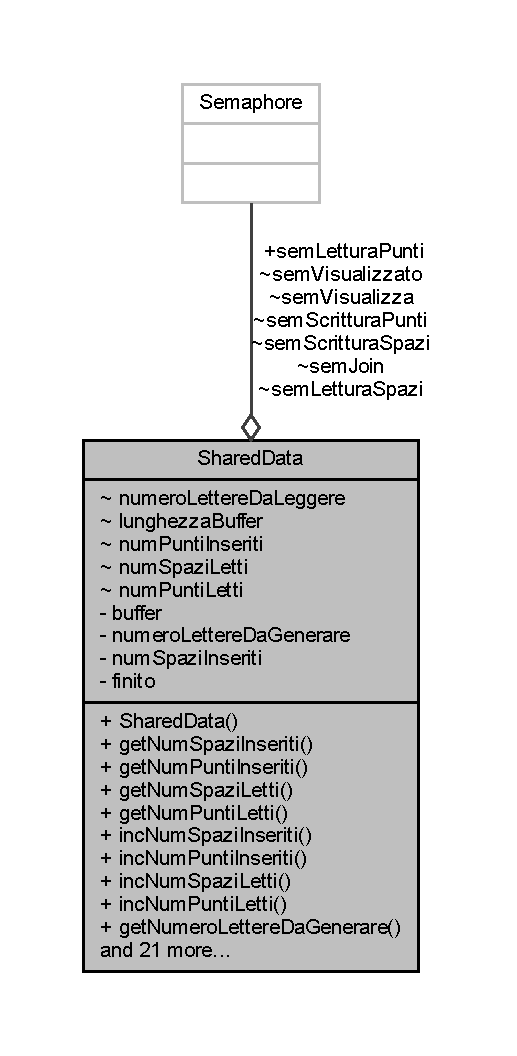
\includegraphics[width=248pt]{classmain_1_1_shared_data__coll__graph}
\end{center}
\end{figure}
\subsection*{Public Member Functions}
\begin{DoxyCompactItemize}
\item 
\mbox{\hyperlink{classmain_1_1_shared_data_a7db3c762818109c4adffd587197cc04c}{Shared\+Data}} (int num)
\item 
int \mbox{\hyperlink{classmain_1_1_shared_data_adc76b1379d370fdffb139d532a622360}{get\+Num\+Spazi\+Inseriti}} ()
\item 
int \mbox{\hyperlink{classmain_1_1_shared_data_a605b5ca567b3e27a318d25b422eaf0a8}{get\+Num\+Punti\+Inseriti}} ()
\item 
int \mbox{\hyperlink{classmain_1_1_shared_data_a54eb961c8dee642d24f9e725eb039827}{get\+Num\+Spazi\+Letti}} ()
\item 
int \mbox{\hyperlink{classmain_1_1_shared_data_ada99c4b55a94591cbe74273d43d7171e}{get\+Num\+Punti\+Letti}} ()
\item 
synchronized void \mbox{\hyperlink{classmain_1_1_shared_data_a5d5262bdb021b4f0deab8fefdb4dfe40}{inc\+Num\+Spazi\+Inseriti}} ()
\item 
synchronized void \mbox{\hyperlink{classmain_1_1_shared_data_a34af1e216aea720d07a45ca716b8893b}{inc\+Num\+Punti\+Inseriti}} ()
\item 
synchronized void \mbox{\hyperlink{classmain_1_1_shared_data_a437c60e2bd2e1647fc60ed8ec7f6616e}{inc\+Num\+Spazi\+Letti}} ()
\item 
synchronized void \mbox{\hyperlink{classmain_1_1_shared_data_aa3c9cc591cbe753063e4dd75f20cfade}{inc\+Num\+Punti\+Letti}} ()
\item 
synchronized int \mbox{\hyperlink{classmain_1_1_shared_data_a7400b59cc3ba24fdb82489e16d602c92}{get\+Numero\+Lettere\+Da\+Generare}} ()
\item 
synchronized void \mbox{\hyperlink{classmain_1_1_shared_data_a9f3f5eba6133dccc829f4e67b23cdfae}{set\+Numero\+Lettere\+Da\+Generare}} (int \mbox{\hyperlink{classmain_1_1_shared_data_a45366d93f9e9d909697e5a38c3449a5c}{numero\+Lettere\+Da\+Generare}})
\item 
synchronized int \mbox{\hyperlink{classmain_1_1_shared_data_a560577008f849ccb788cc398fce280d1}{get\+Numero\+Lettere\+Da\+Leggere}} ()
\item 
synchronized void \mbox{\hyperlink{classmain_1_1_shared_data_aac2fca4598933f3179d78fe7857aed55}{set\+Numero\+Lettere\+Da\+Leggere}} (int numero\+Lettere\+Da\+Leggere)
\item 
synchronized int \mbox{\hyperlink{classmain_1_1_shared_data_a2f606346e7f2ae2e2da2ad211c0bf08a}{get\+Lunghezza\+Buffer}} ()
\item 
synchronized void \mbox{\hyperlink{classmain_1_1_shared_data_a9f4674222bb12c6275156d82033cf17c}{set\+Lunghezza\+Buffer}} (int lunghezza\+Buffer)
\item 
synchronized char \mbox{[}$\,$\mbox{]} \mbox{\hyperlink{classmain_1_1_shared_data_a834679087d3e57272392eaf389f13a80}{get\+Buffer}} ()
\item 
synchronized void \mbox{\hyperlink{classmain_1_1_shared_data_a72a099def4ea0fd3499ed5b33a493245}{set\+Buffer\+At}} (int index, char val)
\item 
synchronized char \mbox{\hyperlink{classmain_1_1_shared_data_acdbb1bf0749f6d59ec74661b16cb10f7}{get\+Buffer\+At}} (int index)
\item 
synchronized void \mbox{\hyperlink{classmain_1_1_shared_data_a00aedde57a20e2963ebc672ae9ce97d4}{clear\+Buffer}} ()
\item 
synchronized void \mbox{\hyperlink{classmain_1_1_shared_data_a0e899cc4037a80b857974e1b46c208bf}{visualizza}} ()
\item 
synchronized boolean \mbox{\hyperlink{classmain_1_1_shared_data_ae7e5f776048f84d07787d62c1ddcf7d0}{is\+Estrazione\+Terminata}} ()
\item 
synchronized void \mbox{\hyperlink{classmain_1_1_shared_data_a7e4be6ed2e568675410bd1666d4bad43}{set\+Estrazione\+Terminata}} (boolean estrazione\+Terminata)
\item 
synchronized boolean \mbox{\hyperlink{classmain_1_1_shared_data_a1cd83a707b62e4056055fd1c6ebba2b0}{is\+Ricerca\+Terminata}} ()
\item 
synchronized void \mbox{\hyperlink{classmain_1_1_shared_data_a8fb1402b905776d228577eee7cdb826f}{set\+Ricerca\+Terminata}} (boolean val, boolean index)
\item 
synchronized Semaphore \mbox{\hyperlink{classmain_1_1_shared_data_a3635e525daf3f0e52187d20e37c90f68}{get\+Sem\+Lettura\+Punti}} ()
\item 
synchronized Semaphore \mbox{\hyperlink{classmain_1_1_shared_data_a218db8263ccc5317ba83f2e4ad2d49c8}{get\+Sem\+Lettura\+Spazi}} ()
\item 
synchronized Semaphore \mbox{\hyperlink{classmain_1_1_shared_data_ae0afb630593f701a83c77bc1ecc12e7b}{get\+Sem\+Scrittura\+Punti}} ()
\item 
synchronized Semaphore \mbox{\hyperlink{classmain_1_1_shared_data_a10670dfbf4c72ab35617e5ee0d73271d}{get\+Sem\+Scrittura\+Spazi}} ()
\item 
synchronized Semaphore \mbox{\hyperlink{classmain_1_1_shared_data_aa61763e3e67d28f279815eda9e81e0bd}{get\+Sem\+Visualizza}} ()
\item 
synchronized Semaphore \mbox{\hyperlink{classmain_1_1_shared_data_a3bc58a39321bc72c013baca2abb19a0a}{get\+Sem\+Visualizzato}} ()
\item 
synchronized Semaphore \mbox{\hyperlink{classmain_1_1_shared_data_a853d0d6001de0c0e8f81c9ab5020c292}{get\+Sem\+Join}} ()
\end{DoxyCompactItemize}
\subsection*{Public Attributes}
\begin{DoxyCompactItemize}
\item 
Semaphore \mbox{\hyperlink{classmain_1_1_shared_data_a524a290baf668c047ed33ad24d49486b}{sem\+Lettura\+Punti}}
\end{DoxyCompactItemize}
\subsection*{Private Attributes}
\begin{DoxyCompactItemize}
\item 
char \mbox{[}$\,$\mbox{]} \mbox{\hyperlink{classmain_1_1_shared_data_a8317b33b8c004741d95935199d964be9}{buffer}}
\item 
int \mbox{\hyperlink{classmain_1_1_shared_data_a45366d93f9e9d909697e5a38c3449a5c}{numero\+Lettere\+Da\+Generare}}
\item 
int \mbox{\hyperlink{classmain_1_1_shared_data_a06a30a83fd49863012db9229233a62eb}{num\+Spazi\+Inseriti}}
\item 
final boolean \mbox{[}$\,$\mbox{]} \mbox{\hyperlink{classmain_1_1_shared_data_a4c4aa548c3dff981a9d44074eaddc93f}{finito}}
\end{DoxyCompactItemize}


\subsection{Detailed Description}
\begin{DoxyAuthor}{Author}
mantica\+\_\+luca 
\end{DoxyAuthor}


Definition at line 14 of file Shared\+Data.\+java.



\subsection{Constructor \& Destructor Documentation}
\mbox{\Hypertarget{classmain_1_1_shared_data_a7db3c762818109c4adffd587197cc04c}\label{classmain_1_1_shared_data_a7db3c762818109c4adffd587197cc04c}} 
\index{main\+::\+Shared\+Data@{main\+::\+Shared\+Data}!Shared\+Data@{Shared\+Data}}
\index{Shared\+Data@{Shared\+Data}!main\+::\+Shared\+Data@{main\+::\+Shared\+Data}}
\subsubsection{\texorpdfstring{Shared\+Data()}{SharedData()}}
{\footnotesize\ttfamily \mbox{\hyperlink{classmain_1_1_shared_data}{Shared\+Data}} (\begin{DoxyParamCaption}\item[{int}]{num }\end{DoxyParamCaption})}



Definition at line 23 of file Shared\+Data.\+java.



\subsection{Member Function Documentation}
\mbox{\Hypertarget{classmain_1_1_shared_data_a00aedde57a20e2963ebc672ae9ce97d4}\label{classmain_1_1_shared_data_a00aedde57a20e2963ebc672ae9ce97d4}} 
\index{main\+::\+Shared\+Data@{main\+::\+Shared\+Data}!clear\+Buffer@{clear\+Buffer}}
\index{clear\+Buffer@{clear\+Buffer}!main\+::\+Shared\+Data@{main\+::\+Shared\+Data}}
\subsubsection{\texorpdfstring{clear\+Buffer()}{clearBuffer()}}
{\footnotesize\ttfamily synchronized void clear\+Buffer (\begin{DoxyParamCaption}{ }\end{DoxyParamCaption})}



Definition at line 111 of file Shared\+Data.\+java.

Here is the caller graph for this function\+:
\nopagebreak
\begin{figure}[H]
\begin{center}
\leavevmode
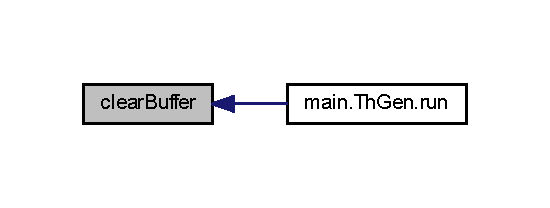
\includegraphics[width=264pt]{classmain_1_1_shared_data_a00aedde57a20e2963ebc672ae9ce97d4_icgraph}
\end{center}
\end{figure}
\mbox{\Hypertarget{classmain_1_1_shared_data_a834679087d3e57272392eaf389f13a80}\label{classmain_1_1_shared_data_a834679087d3e57272392eaf389f13a80}} 
\index{main\+::\+Shared\+Data@{main\+::\+Shared\+Data}!get\+Buffer@{get\+Buffer}}
\index{get\+Buffer@{get\+Buffer}!main\+::\+Shared\+Data@{main\+::\+Shared\+Data}}
\subsubsection{\texorpdfstring{get\+Buffer()}{getBuffer()}}
{\footnotesize\ttfamily synchronized char \mbox{[}$\,$\mbox{]} get\+Buffer (\begin{DoxyParamCaption}{ }\end{DoxyParamCaption})}



Definition at line 99 of file Shared\+Data.\+java.

\mbox{\Hypertarget{classmain_1_1_shared_data_acdbb1bf0749f6d59ec74661b16cb10f7}\label{classmain_1_1_shared_data_acdbb1bf0749f6d59ec74661b16cb10f7}} 
\index{main\+::\+Shared\+Data@{main\+::\+Shared\+Data}!get\+Buffer\+At@{get\+Buffer\+At}}
\index{get\+Buffer\+At@{get\+Buffer\+At}!main\+::\+Shared\+Data@{main\+::\+Shared\+Data}}
\subsubsection{\texorpdfstring{get\+Buffer\+At()}{getBufferAt()}}
{\footnotesize\ttfamily synchronized char get\+Buffer\+At (\begin{DoxyParamCaption}\item[{int}]{index }\end{DoxyParamCaption})}



Definition at line 107 of file Shared\+Data.\+java.

Here is the caller graph for this function\+:
\nopagebreak
\begin{figure}[H]
\begin{center}
\leavevmode
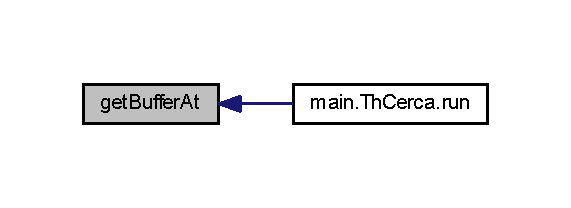
\includegraphics[width=274pt]{classmain_1_1_shared_data_acdbb1bf0749f6d59ec74661b16cb10f7_icgraph}
\end{center}
\end{figure}
\mbox{\Hypertarget{classmain_1_1_shared_data_a2f606346e7f2ae2e2da2ad211c0bf08a}\label{classmain_1_1_shared_data_a2f606346e7f2ae2e2da2ad211c0bf08a}} 
\index{main\+::\+Shared\+Data@{main\+::\+Shared\+Data}!get\+Lunghezza\+Buffer@{get\+Lunghezza\+Buffer}}
\index{get\+Lunghezza\+Buffer@{get\+Lunghezza\+Buffer}!main\+::\+Shared\+Data@{main\+::\+Shared\+Data}}
\subsubsection{\texorpdfstring{get\+Lunghezza\+Buffer()}{getLunghezzaBuffer()}}
{\footnotesize\ttfamily synchronized int get\+Lunghezza\+Buffer (\begin{DoxyParamCaption}{ }\end{DoxyParamCaption})}



Definition at line 91 of file Shared\+Data.\+java.

Here is the caller graph for this function\+:
\nopagebreak
\begin{figure}[H]
\begin{center}
\leavevmode
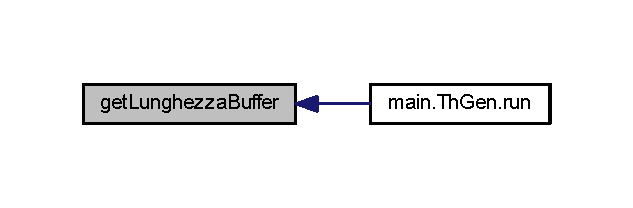
\includegraphics[width=304pt]{classmain_1_1_shared_data_a2f606346e7f2ae2e2da2ad211c0bf08a_icgraph}
\end{center}
\end{figure}
\mbox{\Hypertarget{classmain_1_1_shared_data_a7400b59cc3ba24fdb82489e16d602c92}\label{classmain_1_1_shared_data_a7400b59cc3ba24fdb82489e16d602c92}} 
\index{main\+::\+Shared\+Data@{main\+::\+Shared\+Data}!get\+Numero\+Lettere\+Da\+Generare@{get\+Numero\+Lettere\+Da\+Generare}}
\index{get\+Numero\+Lettere\+Da\+Generare@{get\+Numero\+Lettere\+Da\+Generare}!main\+::\+Shared\+Data@{main\+::\+Shared\+Data}}
\subsubsection{\texorpdfstring{get\+Numero\+Lettere\+Da\+Generare()}{getNumeroLettereDaGenerare()}}
{\footnotesize\ttfamily synchronized int get\+Numero\+Lettere\+Da\+Generare (\begin{DoxyParamCaption}{ }\end{DoxyParamCaption})}



Definition at line 75 of file Shared\+Data.\+java.

Here is the caller graph for this function\+:
\nopagebreak
\begin{figure}[H]
\begin{center}
\leavevmode
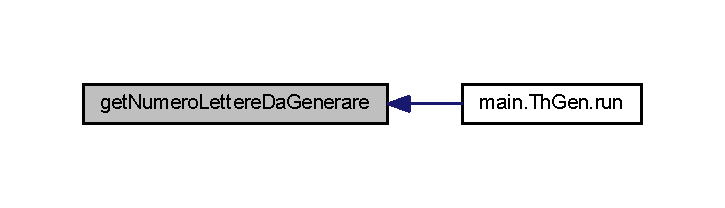
\includegraphics[width=348pt]{classmain_1_1_shared_data_a7400b59cc3ba24fdb82489e16d602c92_icgraph}
\end{center}
\end{figure}
\mbox{\Hypertarget{classmain_1_1_shared_data_a560577008f849ccb788cc398fce280d1}\label{classmain_1_1_shared_data_a560577008f849ccb788cc398fce280d1}} 
\index{main\+::\+Shared\+Data@{main\+::\+Shared\+Data}!get\+Numero\+Lettere\+Da\+Leggere@{get\+Numero\+Lettere\+Da\+Leggere}}
\index{get\+Numero\+Lettere\+Da\+Leggere@{get\+Numero\+Lettere\+Da\+Leggere}!main\+::\+Shared\+Data@{main\+::\+Shared\+Data}}
\subsubsection{\texorpdfstring{get\+Numero\+Lettere\+Da\+Leggere()}{getNumeroLettereDaLeggere()}}
{\footnotesize\ttfamily synchronized int get\+Numero\+Lettere\+Da\+Leggere (\begin{DoxyParamCaption}{ }\end{DoxyParamCaption})}



Definition at line 83 of file Shared\+Data.\+java.

Here is the caller graph for this function\+:
\nopagebreak
\begin{figure}[H]
\begin{center}
\leavevmode
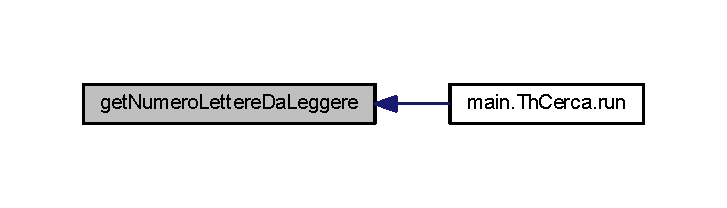
\includegraphics[width=349pt]{classmain_1_1_shared_data_a560577008f849ccb788cc398fce280d1_icgraph}
\end{center}
\end{figure}
\mbox{\Hypertarget{classmain_1_1_shared_data_a605b5ca567b3e27a318d25b422eaf0a8}\label{classmain_1_1_shared_data_a605b5ca567b3e27a318d25b422eaf0a8}} 
\index{main\+::\+Shared\+Data@{main\+::\+Shared\+Data}!get\+Num\+Punti\+Inseriti@{get\+Num\+Punti\+Inseriti}}
\index{get\+Num\+Punti\+Inseriti@{get\+Num\+Punti\+Inseriti}!main\+::\+Shared\+Data@{main\+::\+Shared\+Data}}
\subsubsection{\texorpdfstring{get\+Num\+Punti\+Inseriti()}{getNumPuntiInseriti()}}
{\footnotesize\ttfamily int get\+Num\+Punti\+Inseriti (\begin{DoxyParamCaption}{ }\end{DoxyParamCaption})}



Definition at line 47 of file Shared\+Data.\+java.

Here is the caller graph for this function\+:
\nopagebreak
\begin{figure}[H]
\begin{center}
\leavevmode
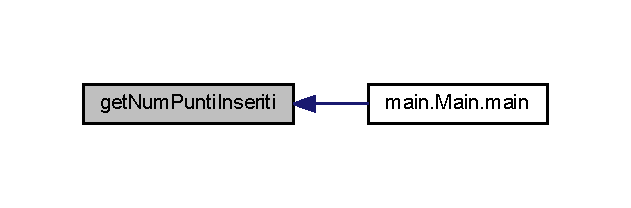
\includegraphics[width=303pt]{classmain_1_1_shared_data_a605b5ca567b3e27a318d25b422eaf0a8_icgraph}
\end{center}
\end{figure}
\mbox{\Hypertarget{classmain_1_1_shared_data_ada99c4b55a94591cbe74273d43d7171e}\label{classmain_1_1_shared_data_ada99c4b55a94591cbe74273d43d7171e}} 
\index{main\+::\+Shared\+Data@{main\+::\+Shared\+Data}!get\+Num\+Punti\+Letti@{get\+Num\+Punti\+Letti}}
\index{get\+Num\+Punti\+Letti@{get\+Num\+Punti\+Letti}!main\+::\+Shared\+Data@{main\+::\+Shared\+Data}}
\subsubsection{\texorpdfstring{get\+Num\+Punti\+Letti()}{getNumPuntiLetti()}}
{\footnotesize\ttfamily int get\+Num\+Punti\+Letti (\begin{DoxyParamCaption}{ }\end{DoxyParamCaption})}



Definition at line 55 of file Shared\+Data.\+java.

Here is the caller graph for this function\+:
\nopagebreak
\begin{figure}[H]
\begin{center}
\leavevmode
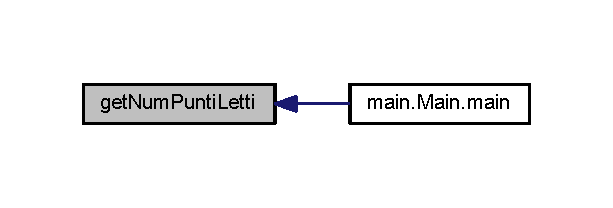
\includegraphics[width=294pt]{classmain_1_1_shared_data_ada99c4b55a94591cbe74273d43d7171e_icgraph}
\end{center}
\end{figure}
\mbox{\Hypertarget{classmain_1_1_shared_data_adc76b1379d370fdffb139d532a622360}\label{classmain_1_1_shared_data_adc76b1379d370fdffb139d532a622360}} 
\index{main\+::\+Shared\+Data@{main\+::\+Shared\+Data}!get\+Num\+Spazi\+Inseriti@{get\+Num\+Spazi\+Inseriti}}
\index{get\+Num\+Spazi\+Inseriti@{get\+Num\+Spazi\+Inseriti}!main\+::\+Shared\+Data@{main\+::\+Shared\+Data}}
\subsubsection{\texorpdfstring{get\+Num\+Spazi\+Inseriti()}{getNumSpaziInseriti()}}
{\footnotesize\ttfamily int get\+Num\+Spazi\+Inseriti (\begin{DoxyParamCaption}{ }\end{DoxyParamCaption})}



Definition at line 43 of file Shared\+Data.\+java.

Here is the caller graph for this function\+:
\nopagebreak
\begin{figure}[H]
\begin{center}
\leavevmode
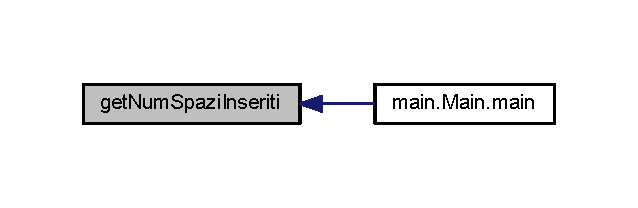
\includegraphics[width=306pt]{classmain_1_1_shared_data_adc76b1379d370fdffb139d532a622360_icgraph}
\end{center}
\end{figure}
\mbox{\Hypertarget{classmain_1_1_shared_data_a54eb961c8dee642d24f9e725eb039827}\label{classmain_1_1_shared_data_a54eb961c8dee642d24f9e725eb039827}} 
\index{main\+::\+Shared\+Data@{main\+::\+Shared\+Data}!get\+Num\+Spazi\+Letti@{get\+Num\+Spazi\+Letti}}
\index{get\+Num\+Spazi\+Letti@{get\+Num\+Spazi\+Letti}!main\+::\+Shared\+Data@{main\+::\+Shared\+Data}}
\subsubsection{\texorpdfstring{get\+Num\+Spazi\+Letti()}{getNumSpaziLetti()}}
{\footnotesize\ttfamily int get\+Num\+Spazi\+Letti (\begin{DoxyParamCaption}{ }\end{DoxyParamCaption})}



Definition at line 51 of file Shared\+Data.\+java.

Here is the caller graph for this function\+:
\nopagebreak
\begin{figure}[H]
\begin{center}
\leavevmode
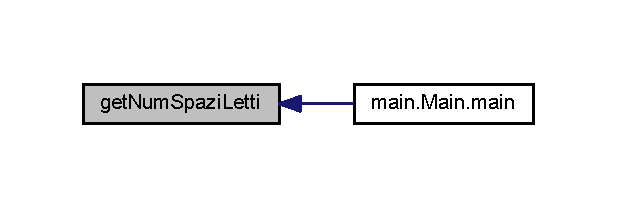
\includegraphics[width=296pt]{classmain_1_1_shared_data_a54eb961c8dee642d24f9e725eb039827_icgraph}
\end{center}
\end{figure}
\mbox{\Hypertarget{classmain_1_1_shared_data_a853d0d6001de0c0e8f81c9ab5020c292}\label{classmain_1_1_shared_data_a853d0d6001de0c0e8f81c9ab5020c292}} 
\index{main\+::\+Shared\+Data@{main\+::\+Shared\+Data}!get\+Sem\+Join@{get\+Sem\+Join}}
\index{get\+Sem\+Join@{get\+Sem\+Join}!main\+::\+Shared\+Data@{main\+::\+Shared\+Data}}
\subsubsection{\texorpdfstring{get\+Sem\+Join()}{getSemJoin()}}
{\footnotesize\ttfamily synchronized Semaphore get\+Sem\+Join (\begin{DoxyParamCaption}{ }\end{DoxyParamCaption})}



Definition at line 164 of file Shared\+Data.\+java.

Here is the caller graph for this function\+:
\nopagebreak
\begin{figure}[H]
\begin{center}
\leavevmode
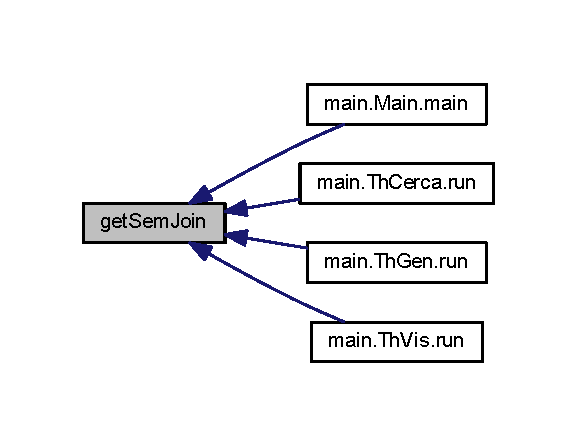
\includegraphics[width=277pt]{classmain_1_1_shared_data_a853d0d6001de0c0e8f81c9ab5020c292_icgraph}
\end{center}
\end{figure}
\mbox{\Hypertarget{classmain_1_1_shared_data_a3635e525daf3f0e52187d20e37c90f68}\label{classmain_1_1_shared_data_a3635e525daf3f0e52187d20e37c90f68}} 
\index{main\+::\+Shared\+Data@{main\+::\+Shared\+Data}!get\+Sem\+Lettura\+Punti@{get\+Sem\+Lettura\+Punti}}
\index{get\+Sem\+Lettura\+Punti@{get\+Sem\+Lettura\+Punti}!main\+::\+Shared\+Data@{main\+::\+Shared\+Data}}
\subsubsection{\texorpdfstring{get\+Sem\+Lettura\+Punti()}{getSemLetturaPunti()}}
{\footnotesize\ttfamily synchronized Semaphore get\+Sem\+Lettura\+Punti (\begin{DoxyParamCaption}{ }\end{DoxyParamCaption})}



Definition at line 140 of file Shared\+Data.\+java.

Here is the caller graph for this function\+:
\nopagebreak
\begin{figure}[H]
\begin{center}
\leavevmode
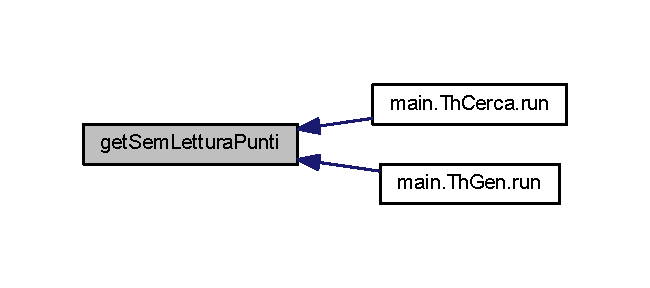
\includegraphics[width=312pt]{classmain_1_1_shared_data_a3635e525daf3f0e52187d20e37c90f68_icgraph}
\end{center}
\end{figure}
\mbox{\Hypertarget{classmain_1_1_shared_data_a218db8263ccc5317ba83f2e4ad2d49c8}\label{classmain_1_1_shared_data_a218db8263ccc5317ba83f2e4ad2d49c8}} 
\index{main\+::\+Shared\+Data@{main\+::\+Shared\+Data}!get\+Sem\+Lettura\+Spazi@{get\+Sem\+Lettura\+Spazi}}
\index{get\+Sem\+Lettura\+Spazi@{get\+Sem\+Lettura\+Spazi}!main\+::\+Shared\+Data@{main\+::\+Shared\+Data}}
\subsubsection{\texorpdfstring{get\+Sem\+Lettura\+Spazi()}{getSemLetturaSpazi()}}
{\footnotesize\ttfamily synchronized Semaphore get\+Sem\+Lettura\+Spazi (\begin{DoxyParamCaption}{ }\end{DoxyParamCaption})}



Definition at line 144 of file Shared\+Data.\+java.

Here is the caller graph for this function\+:
\nopagebreak
\begin{figure}[H]
\begin{center}
\leavevmode
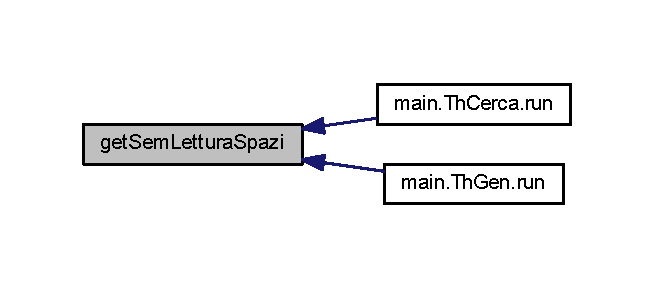
\includegraphics[width=314pt]{classmain_1_1_shared_data_a218db8263ccc5317ba83f2e4ad2d49c8_icgraph}
\end{center}
\end{figure}
\mbox{\Hypertarget{classmain_1_1_shared_data_ae0afb630593f701a83c77bc1ecc12e7b}\label{classmain_1_1_shared_data_ae0afb630593f701a83c77bc1ecc12e7b}} 
\index{main\+::\+Shared\+Data@{main\+::\+Shared\+Data}!get\+Sem\+Scrittura\+Punti@{get\+Sem\+Scrittura\+Punti}}
\index{get\+Sem\+Scrittura\+Punti@{get\+Sem\+Scrittura\+Punti}!main\+::\+Shared\+Data@{main\+::\+Shared\+Data}}
\subsubsection{\texorpdfstring{get\+Sem\+Scrittura\+Punti()}{getSemScritturaPunti()}}
{\footnotesize\ttfamily synchronized Semaphore get\+Sem\+Scrittura\+Punti (\begin{DoxyParamCaption}{ }\end{DoxyParamCaption})}



Definition at line 148 of file Shared\+Data.\+java.

Here is the caller graph for this function\+:
\nopagebreak
\begin{figure}[H]
\begin{center}
\leavevmode
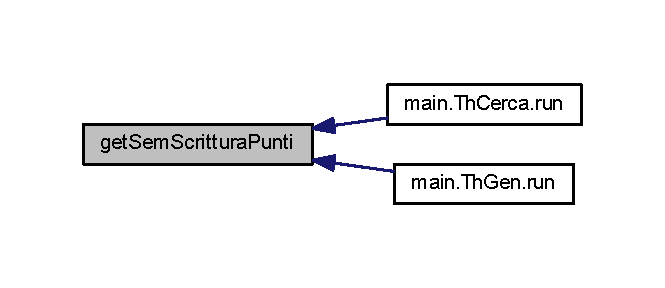
\includegraphics[width=319pt]{classmain_1_1_shared_data_ae0afb630593f701a83c77bc1ecc12e7b_icgraph}
\end{center}
\end{figure}
\mbox{\Hypertarget{classmain_1_1_shared_data_a10670dfbf4c72ab35617e5ee0d73271d}\label{classmain_1_1_shared_data_a10670dfbf4c72ab35617e5ee0d73271d}} 
\index{main\+::\+Shared\+Data@{main\+::\+Shared\+Data}!get\+Sem\+Scrittura\+Spazi@{get\+Sem\+Scrittura\+Spazi}}
\index{get\+Sem\+Scrittura\+Spazi@{get\+Sem\+Scrittura\+Spazi}!main\+::\+Shared\+Data@{main\+::\+Shared\+Data}}
\subsubsection{\texorpdfstring{get\+Sem\+Scrittura\+Spazi()}{getSemScritturaSpazi()}}
{\footnotesize\ttfamily synchronized Semaphore get\+Sem\+Scrittura\+Spazi (\begin{DoxyParamCaption}{ }\end{DoxyParamCaption})}



Definition at line 152 of file Shared\+Data.\+java.

Here is the caller graph for this function\+:
\nopagebreak
\begin{figure}[H]
\begin{center}
\leavevmode
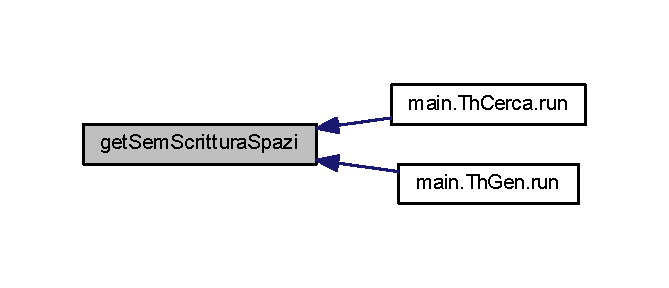
\includegraphics[width=321pt]{classmain_1_1_shared_data_a10670dfbf4c72ab35617e5ee0d73271d_icgraph}
\end{center}
\end{figure}
\mbox{\Hypertarget{classmain_1_1_shared_data_aa61763e3e67d28f279815eda9e81e0bd}\label{classmain_1_1_shared_data_aa61763e3e67d28f279815eda9e81e0bd}} 
\index{main\+::\+Shared\+Data@{main\+::\+Shared\+Data}!get\+Sem\+Visualizza@{get\+Sem\+Visualizza}}
\index{get\+Sem\+Visualizza@{get\+Sem\+Visualizza}!main\+::\+Shared\+Data@{main\+::\+Shared\+Data}}
\subsubsection{\texorpdfstring{get\+Sem\+Visualizza()}{getSemVisualizza()}}
{\footnotesize\ttfamily synchronized Semaphore get\+Sem\+Visualizza (\begin{DoxyParamCaption}{ }\end{DoxyParamCaption})}



Definition at line 156 of file Shared\+Data.\+java.

Here is the caller graph for this function\+:
\nopagebreak
\begin{figure}[H]
\begin{center}
\leavevmode
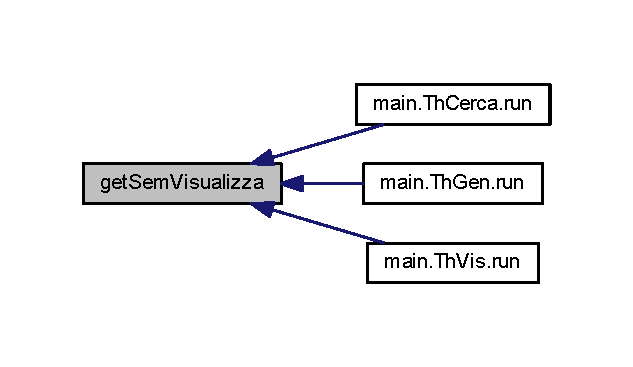
\includegraphics[width=304pt]{classmain_1_1_shared_data_aa61763e3e67d28f279815eda9e81e0bd_icgraph}
\end{center}
\end{figure}
\mbox{\Hypertarget{classmain_1_1_shared_data_a3bc58a39321bc72c013baca2abb19a0a}\label{classmain_1_1_shared_data_a3bc58a39321bc72c013baca2abb19a0a}} 
\index{main\+::\+Shared\+Data@{main\+::\+Shared\+Data}!get\+Sem\+Visualizzato@{get\+Sem\+Visualizzato}}
\index{get\+Sem\+Visualizzato@{get\+Sem\+Visualizzato}!main\+::\+Shared\+Data@{main\+::\+Shared\+Data}}
\subsubsection{\texorpdfstring{get\+Sem\+Visualizzato()}{getSemVisualizzato()}}
{\footnotesize\ttfamily synchronized Semaphore get\+Sem\+Visualizzato (\begin{DoxyParamCaption}{ }\end{DoxyParamCaption})}



Definition at line 160 of file Shared\+Data.\+java.

Here is the caller graph for this function\+:
\nopagebreak
\begin{figure}[H]
\begin{center}
\leavevmode
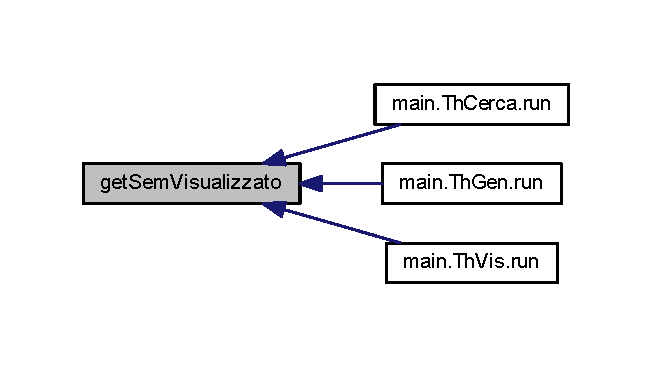
\includegraphics[width=313pt]{classmain_1_1_shared_data_a3bc58a39321bc72c013baca2abb19a0a_icgraph}
\end{center}
\end{figure}
\mbox{\Hypertarget{classmain_1_1_shared_data_a34af1e216aea720d07a45ca716b8893b}\label{classmain_1_1_shared_data_a34af1e216aea720d07a45ca716b8893b}} 
\index{main\+::\+Shared\+Data@{main\+::\+Shared\+Data}!inc\+Num\+Punti\+Inseriti@{inc\+Num\+Punti\+Inseriti}}
\index{inc\+Num\+Punti\+Inseriti@{inc\+Num\+Punti\+Inseriti}!main\+::\+Shared\+Data@{main\+::\+Shared\+Data}}
\subsubsection{\texorpdfstring{inc\+Num\+Punti\+Inseriti()}{incNumPuntiInseriti()}}
{\footnotesize\ttfamily synchronized void inc\+Num\+Punti\+Inseriti (\begin{DoxyParamCaption}{ }\end{DoxyParamCaption})}



Definition at line 63 of file Shared\+Data.\+java.

Here is the caller graph for this function\+:
\nopagebreak
\begin{figure}[H]
\begin{center}
\leavevmode
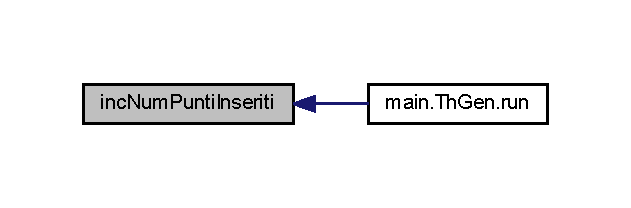
\includegraphics[width=303pt]{classmain_1_1_shared_data_a34af1e216aea720d07a45ca716b8893b_icgraph}
\end{center}
\end{figure}
\mbox{\Hypertarget{classmain_1_1_shared_data_aa3c9cc591cbe753063e4dd75f20cfade}\label{classmain_1_1_shared_data_aa3c9cc591cbe753063e4dd75f20cfade}} 
\index{main\+::\+Shared\+Data@{main\+::\+Shared\+Data}!inc\+Num\+Punti\+Letti@{inc\+Num\+Punti\+Letti}}
\index{inc\+Num\+Punti\+Letti@{inc\+Num\+Punti\+Letti}!main\+::\+Shared\+Data@{main\+::\+Shared\+Data}}
\subsubsection{\texorpdfstring{inc\+Num\+Punti\+Letti()}{incNumPuntiLetti()}}
{\footnotesize\ttfamily synchronized void inc\+Num\+Punti\+Letti (\begin{DoxyParamCaption}{ }\end{DoxyParamCaption})}



Definition at line 71 of file Shared\+Data.\+java.

Here is the caller graph for this function\+:
\nopagebreak
\begin{figure}[H]
\begin{center}
\leavevmode
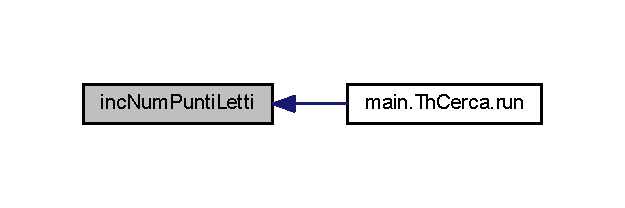
\includegraphics[width=300pt]{classmain_1_1_shared_data_aa3c9cc591cbe753063e4dd75f20cfade_icgraph}
\end{center}
\end{figure}
\mbox{\Hypertarget{classmain_1_1_shared_data_a5d5262bdb021b4f0deab8fefdb4dfe40}\label{classmain_1_1_shared_data_a5d5262bdb021b4f0deab8fefdb4dfe40}} 
\index{main\+::\+Shared\+Data@{main\+::\+Shared\+Data}!inc\+Num\+Spazi\+Inseriti@{inc\+Num\+Spazi\+Inseriti}}
\index{inc\+Num\+Spazi\+Inseriti@{inc\+Num\+Spazi\+Inseriti}!main\+::\+Shared\+Data@{main\+::\+Shared\+Data}}
\subsubsection{\texorpdfstring{inc\+Num\+Spazi\+Inseriti()}{incNumSpaziInseriti()}}
{\footnotesize\ttfamily synchronized void inc\+Num\+Spazi\+Inseriti (\begin{DoxyParamCaption}{ }\end{DoxyParamCaption})}



Definition at line 59 of file Shared\+Data.\+java.

Here is the caller graph for this function\+:
\nopagebreak
\begin{figure}[H]
\begin{center}
\leavevmode
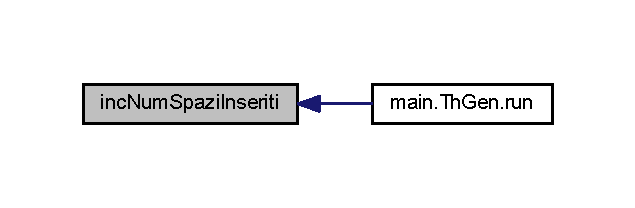
\includegraphics[width=305pt]{classmain_1_1_shared_data_a5d5262bdb021b4f0deab8fefdb4dfe40_icgraph}
\end{center}
\end{figure}
\mbox{\Hypertarget{classmain_1_1_shared_data_a437c60e2bd2e1647fc60ed8ec7f6616e}\label{classmain_1_1_shared_data_a437c60e2bd2e1647fc60ed8ec7f6616e}} 
\index{main\+::\+Shared\+Data@{main\+::\+Shared\+Data}!inc\+Num\+Spazi\+Letti@{inc\+Num\+Spazi\+Letti}}
\index{inc\+Num\+Spazi\+Letti@{inc\+Num\+Spazi\+Letti}!main\+::\+Shared\+Data@{main\+::\+Shared\+Data}}
\subsubsection{\texorpdfstring{inc\+Num\+Spazi\+Letti()}{incNumSpaziLetti()}}
{\footnotesize\ttfamily synchronized void inc\+Num\+Spazi\+Letti (\begin{DoxyParamCaption}{ }\end{DoxyParamCaption})}



Definition at line 67 of file Shared\+Data.\+java.

Here is the caller graph for this function\+:
\nopagebreak
\begin{figure}[H]
\begin{center}
\leavevmode
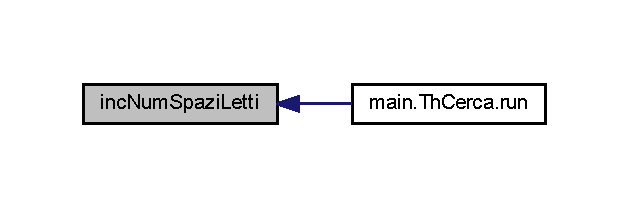
\includegraphics[width=302pt]{classmain_1_1_shared_data_a437c60e2bd2e1647fc60ed8ec7f6616e_icgraph}
\end{center}
\end{figure}
\mbox{\Hypertarget{classmain_1_1_shared_data_ae7e5f776048f84d07787d62c1ddcf7d0}\label{classmain_1_1_shared_data_ae7e5f776048f84d07787d62c1ddcf7d0}} 
\index{main\+::\+Shared\+Data@{main\+::\+Shared\+Data}!is\+Estrazione\+Terminata@{is\+Estrazione\+Terminata}}
\index{is\+Estrazione\+Terminata@{is\+Estrazione\+Terminata}!main\+::\+Shared\+Data@{main\+::\+Shared\+Data}}
\subsubsection{\texorpdfstring{is\+Estrazione\+Terminata()}{isEstrazioneTerminata()}}
{\footnotesize\ttfamily synchronized boolean is\+Estrazione\+Terminata (\begin{DoxyParamCaption}{ }\end{DoxyParamCaption})}



Definition at line 123 of file Shared\+Data.\+java.

Here is the caller graph for this function\+:
\nopagebreak
\begin{figure}[H]
\begin{center}
\leavevmode
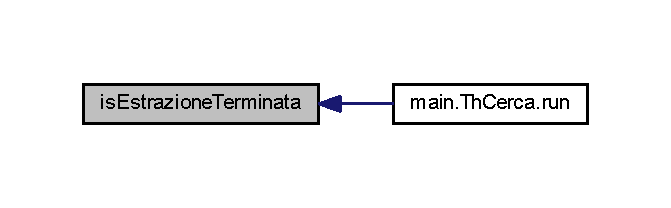
\includegraphics[width=322pt]{classmain_1_1_shared_data_ae7e5f776048f84d07787d62c1ddcf7d0_icgraph}
\end{center}
\end{figure}
\mbox{\Hypertarget{classmain_1_1_shared_data_a1cd83a707b62e4056055fd1c6ebba2b0}\label{classmain_1_1_shared_data_a1cd83a707b62e4056055fd1c6ebba2b0}} 
\index{main\+::\+Shared\+Data@{main\+::\+Shared\+Data}!is\+Ricerca\+Terminata@{is\+Ricerca\+Terminata}}
\index{is\+Ricerca\+Terminata@{is\+Ricerca\+Terminata}!main\+::\+Shared\+Data@{main\+::\+Shared\+Data}}
\subsubsection{\texorpdfstring{is\+Ricerca\+Terminata()}{isRicercaTerminata()}}
{\footnotesize\ttfamily synchronized boolean is\+Ricerca\+Terminata (\begin{DoxyParamCaption}{ }\end{DoxyParamCaption})}



Definition at line 131 of file Shared\+Data.\+java.

Here is the caller graph for this function\+:
\nopagebreak
\begin{figure}[H]
\begin{center}
\leavevmode
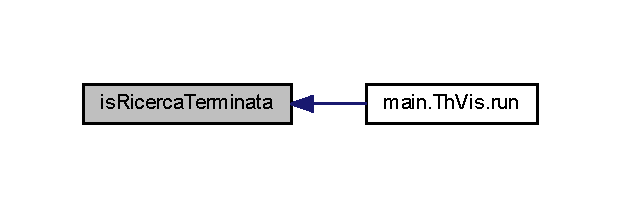
\includegraphics[width=298pt]{classmain_1_1_shared_data_a1cd83a707b62e4056055fd1c6ebba2b0_icgraph}
\end{center}
\end{figure}
\mbox{\Hypertarget{classmain_1_1_shared_data_a72a099def4ea0fd3499ed5b33a493245}\label{classmain_1_1_shared_data_a72a099def4ea0fd3499ed5b33a493245}} 
\index{main\+::\+Shared\+Data@{main\+::\+Shared\+Data}!set\+Buffer\+At@{set\+Buffer\+At}}
\index{set\+Buffer\+At@{set\+Buffer\+At}!main\+::\+Shared\+Data@{main\+::\+Shared\+Data}}
\subsubsection{\texorpdfstring{set\+Buffer\+At()}{setBufferAt()}}
{\footnotesize\ttfamily synchronized void set\+Buffer\+At (\begin{DoxyParamCaption}\item[{int}]{index,  }\item[{char}]{val }\end{DoxyParamCaption})}



Definition at line 103 of file Shared\+Data.\+java.

Here is the caller graph for this function\+:
\nopagebreak
\begin{figure}[H]
\begin{center}
\leavevmode
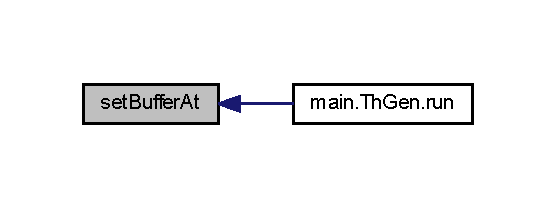
\includegraphics[width=267pt]{classmain_1_1_shared_data_a72a099def4ea0fd3499ed5b33a493245_icgraph}
\end{center}
\end{figure}
\mbox{\Hypertarget{classmain_1_1_shared_data_a7e4be6ed2e568675410bd1666d4bad43}\label{classmain_1_1_shared_data_a7e4be6ed2e568675410bd1666d4bad43}} 
\index{main\+::\+Shared\+Data@{main\+::\+Shared\+Data}!set\+Estrazione\+Terminata@{set\+Estrazione\+Terminata}}
\index{set\+Estrazione\+Terminata@{set\+Estrazione\+Terminata}!main\+::\+Shared\+Data@{main\+::\+Shared\+Data}}
\subsubsection{\texorpdfstring{set\+Estrazione\+Terminata()}{setEstrazioneTerminata()}}
{\footnotesize\ttfamily synchronized void set\+Estrazione\+Terminata (\begin{DoxyParamCaption}\item[{boolean}]{estrazione\+Terminata }\end{DoxyParamCaption})}



Definition at line 127 of file Shared\+Data.\+java.

Here is the caller graph for this function\+:
\nopagebreak
\begin{figure}[H]
\begin{center}
\leavevmode
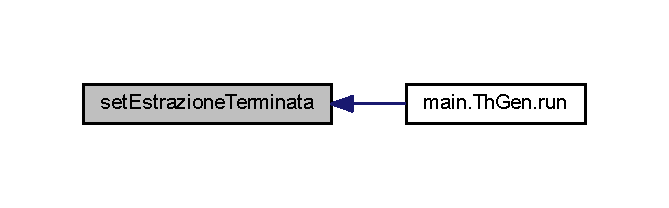
\includegraphics[width=321pt]{classmain_1_1_shared_data_a7e4be6ed2e568675410bd1666d4bad43_icgraph}
\end{center}
\end{figure}
\mbox{\Hypertarget{classmain_1_1_shared_data_a9f4674222bb12c6275156d82033cf17c}\label{classmain_1_1_shared_data_a9f4674222bb12c6275156d82033cf17c}} 
\index{main\+::\+Shared\+Data@{main\+::\+Shared\+Data}!set\+Lunghezza\+Buffer@{set\+Lunghezza\+Buffer}}
\index{set\+Lunghezza\+Buffer@{set\+Lunghezza\+Buffer}!main\+::\+Shared\+Data@{main\+::\+Shared\+Data}}
\subsubsection{\texorpdfstring{set\+Lunghezza\+Buffer()}{setLunghezzaBuffer()}}
{\footnotesize\ttfamily synchronized void set\+Lunghezza\+Buffer (\begin{DoxyParamCaption}\item[{int}]{lunghezza\+Buffer }\end{DoxyParamCaption})}



Definition at line 95 of file Shared\+Data.\+java.

\mbox{\Hypertarget{classmain_1_1_shared_data_a9f3f5eba6133dccc829f4e67b23cdfae}\label{classmain_1_1_shared_data_a9f3f5eba6133dccc829f4e67b23cdfae}} 
\index{main\+::\+Shared\+Data@{main\+::\+Shared\+Data}!set\+Numero\+Lettere\+Da\+Generare@{set\+Numero\+Lettere\+Da\+Generare}}
\index{set\+Numero\+Lettere\+Da\+Generare@{set\+Numero\+Lettere\+Da\+Generare}!main\+::\+Shared\+Data@{main\+::\+Shared\+Data}}
\subsubsection{\texorpdfstring{set\+Numero\+Lettere\+Da\+Generare()}{setNumeroLettereDaGenerare()}}
{\footnotesize\ttfamily synchronized void set\+Numero\+Lettere\+Da\+Generare (\begin{DoxyParamCaption}\item[{int}]{numero\+Lettere\+Da\+Generare }\end{DoxyParamCaption})}



Definition at line 79 of file Shared\+Data.\+java.

\mbox{\Hypertarget{classmain_1_1_shared_data_aac2fca4598933f3179d78fe7857aed55}\label{classmain_1_1_shared_data_aac2fca4598933f3179d78fe7857aed55}} 
\index{main\+::\+Shared\+Data@{main\+::\+Shared\+Data}!set\+Numero\+Lettere\+Da\+Leggere@{set\+Numero\+Lettere\+Da\+Leggere}}
\index{set\+Numero\+Lettere\+Da\+Leggere@{set\+Numero\+Lettere\+Da\+Leggere}!main\+::\+Shared\+Data@{main\+::\+Shared\+Data}}
\subsubsection{\texorpdfstring{set\+Numero\+Lettere\+Da\+Leggere()}{setNumeroLettereDaLeggere()}}
{\footnotesize\ttfamily synchronized void set\+Numero\+Lettere\+Da\+Leggere (\begin{DoxyParamCaption}\item[{int}]{numero\+Lettere\+Da\+Leggere }\end{DoxyParamCaption})}



Definition at line 87 of file Shared\+Data.\+java.

Here is the caller graph for this function\+:
\nopagebreak
\begin{figure}[H]
\begin{center}
\leavevmode
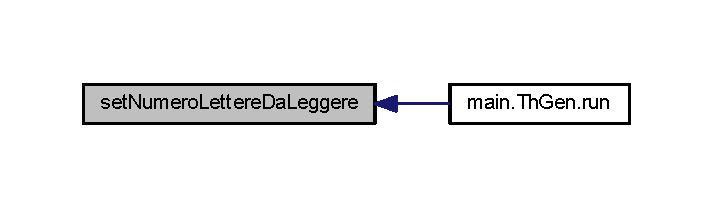
\includegraphics[width=342pt]{classmain_1_1_shared_data_aac2fca4598933f3179d78fe7857aed55_icgraph}
\end{center}
\end{figure}
\mbox{\Hypertarget{classmain_1_1_shared_data_a8fb1402b905776d228577eee7cdb826f}\label{classmain_1_1_shared_data_a8fb1402b905776d228577eee7cdb826f}} 
\index{main\+::\+Shared\+Data@{main\+::\+Shared\+Data}!set\+Ricerca\+Terminata@{set\+Ricerca\+Terminata}}
\index{set\+Ricerca\+Terminata@{set\+Ricerca\+Terminata}!main\+::\+Shared\+Data@{main\+::\+Shared\+Data}}
\subsubsection{\texorpdfstring{set\+Ricerca\+Terminata()}{setRicercaTerminata()}}
{\footnotesize\ttfamily synchronized void set\+Ricerca\+Terminata (\begin{DoxyParamCaption}\item[{boolean}]{val,  }\item[{boolean}]{index }\end{DoxyParamCaption})}



Definition at line 135 of file Shared\+Data.\+java.

Here is the caller graph for this function\+:
\nopagebreak
\begin{figure}[H]
\begin{center}
\leavevmode
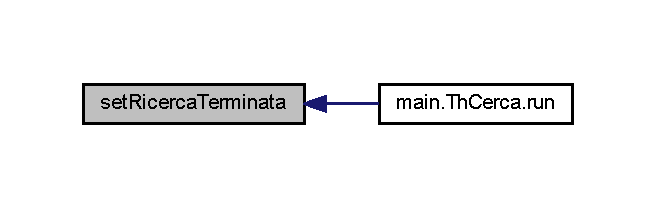
\includegraphics[width=315pt]{classmain_1_1_shared_data_a8fb1402b905776d228577eee7cdb826f_icgraph}
\end{center}
\end{figure}
\mbox{\Hypertarget{classmain_1_1_shared_data_a0e899cc4037a80b857974e1b46c208bf}\label{classmain_1_1_shared_data_a0e899cc4037a80b857974e1b46c208bf}} 
\index{main\+::\+Shared\+Data@{main\+::\+Shared\+Data}!visualizza@{visualizza}}
\index{visualizza@{visualizza}!main\+::\+Shared\+Data@{main\+::\+Shared\+Data}}
\subsubsection{\texorpdfstring{visualizza()}{visualizza()}}
{\footnotesize\ttfamily synchronized void visualizza (\begin{DoxyParamCaption}{ }\end{DoxyParamCaption})}



Definition at line 115 of file Shared\+Data.\+java.

Here is the caller graph for this function\+:
\nopagebreak
\begin{figure}[H]
\begin{center}
\leavevmode
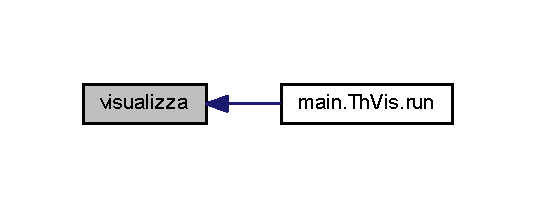
\includegraphics[width=257pt]{classmain_1_1_shared_data_a0e899cc4037a80b857974e1b46c208bf_icgraph}
\end{center}
\end{figure}


\subsection{Member Data Documentation}
\mbox{\Hypertarget{classmain_1_1_shared_data_a8317b33b8c004741d95935199d964be9}\label{classmain_1_1_shared_data_a8317b33b8c004741d95935199d964be9}} 
\index{main\+::\+Shared\+Data@{main\+::\+Shared\+Data}!buffer@{buffer}}
\index{buffer@{buffer}!main\+::\+Shared\+Data@{main\+::\+Shared\+Data}}
\subsubsection{\texorpdfstring{buffer}{buffer}}
{\footnotesize\ttfamily char \mbox{[}$\,$\mbox{]} buffer\hspace{0.3cm}{\ttfamily [private]}}



Definition at line 17 of file Shared\+Data.\+java.

\mbox{\Hypertarget{classmain_1_1_shared_data_a4c4aa548c3dff981a9d44074eaddc93f}\label{classmain_1_1_shared_data_a4c4aa548c3dff981a9d44074eaddc93f}} 
\index{main\+::\+Shared\+Data@{main\+::\+Shared\+Data}!finito@{finito}}
\index{finito@{finito}!main\+::\+Shared\+Data@{main\+::\+Shared\+Data}}
\subsubsection{\texorpdfstring{finito}{finito}}
{\footnotesize\ttfamily final boolean \mbox{[}$\,$\mbox{]} finito\hspace{0.3cm}{\ttfamily [private]}}



Definition at line 21 of file Shared\+Data.\+java.

\mbox{\Hypertarget{classmain_1_1_shared_data_a45366d93f9e9d909697e5a38c3449a5c}\label{classmain_1_1_shared_data_a45366d93f9e9d909697e5a38c3449a5c}} 
\index{main\+::\+Shared\+Data@{main\+::\+Shared\+Data}!numero\+Lettere\+Da\+Generare@{numero\+Lettere\+Da\+Generare}}
\index{numero\+Lettere\+Da\+Generare@{numero\+Lettere\+Da\+Generare}!main\+::\+Shared\+Data@{main\+::\+Shared\+Data}}
\subsubsection{\texorpdfstring{numero\+Lettere\+Da\+Generare}{numeroLettereDaGenerare}}
{\footnotesize\ttfamily int numero\+Lettere\+Da\+Generare\hspace{0.3cm}{\ttfamily [private]}}



Definition at line 18 of file Shared\+Data.\+java.

\mbox{\Hypertarget{classmain_1_1_shared_data_a06a30a83fd49863012db9229233a62eb}\label{classmain_1_1_shared_data_a06a30a83fd49863012db9229233a62eb}} 
\index{main\+::\+Shared\+Data@{main\+::\+Shared\+Data}!num\+Spazi\+Inseriti@{num\+Spazi\+Inseriti}}
\index{num\+Spazi\+Inseriti@{num\+Spazi\+Inseriti}!main\+::\+Shared\+Data@{main\+::\+Shared\+Data}}
\subsubsection{\texorpdfstring{num\+Spazi\+Inseriti}{numSpaziInseriti}}
{\footnotesize\ttfamily int num\+Spazi\+Inseriti\hspace{0.3cm}{\ttfamily [private]}}



Definition at line 19 of file Shared\+Data.\+java.

\mbox{\Hypertarget{classmain_1_1_shared_data_a524a290baf668c047ed33ad24d49486b}\label{classmain_1_1_shared_data_a524a290baf668c047ed33ad24d49486b}} 
\index{main\+::\+Shared\+Data@{main\+::\+Shared\+Data}!sem\+Lettura\+Punti@{sem\+Lettura\+Punti}}
\index{sem\+Lettura\+Punti@{sem\+Lettura\+Punti}!main\+::\+Shared\+Data@{main\+::\+Shared\+Data}}
\subsubsection{\texorpdfstring{sem\+Lettura\+Punti}{semLetturaPunti}}
{\footnotesize\ttfamily Semaphore sem\+Lettura\+Punti}



Definition at line 16 of file Shared\+Data.\+java.



The documentation for this class was generated from the following file\+:\begin{DoxyCompactItemize}
\item 
Statistiche/src/main/\mbox{\hyperlink{_shared_data_8java}{Shared\+Data.\+java}}\end{DoxyCompactItemize}

\hypertarget{classmain_1_1_th_cerca}{}\section{Th\+Cerca Class Reference}
\label{classmain_1_1_th_cerca}\index{Th\+Cerca@{Th\+Cerca}}


Inheritance diagram for Th\+Cerca\+:
\nopagebreak
\begin{figure}[H]
\begin{center}
\leavevmode
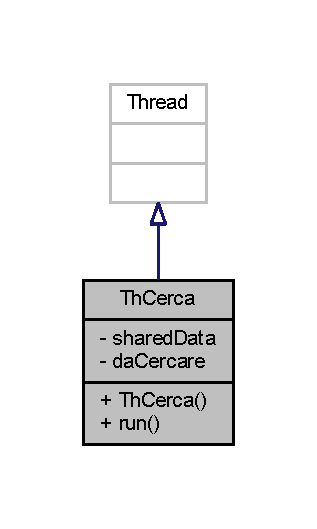
\includegraphics[width=152pt]{classmain_1_1_th_cerca__inherit__graph}
\end{center}
\end{figure}


Collaboration diagram for Th\+Cerca\+:
\nopagebreak
\begin{figure}[H]
\begin{center}
\leavevmode
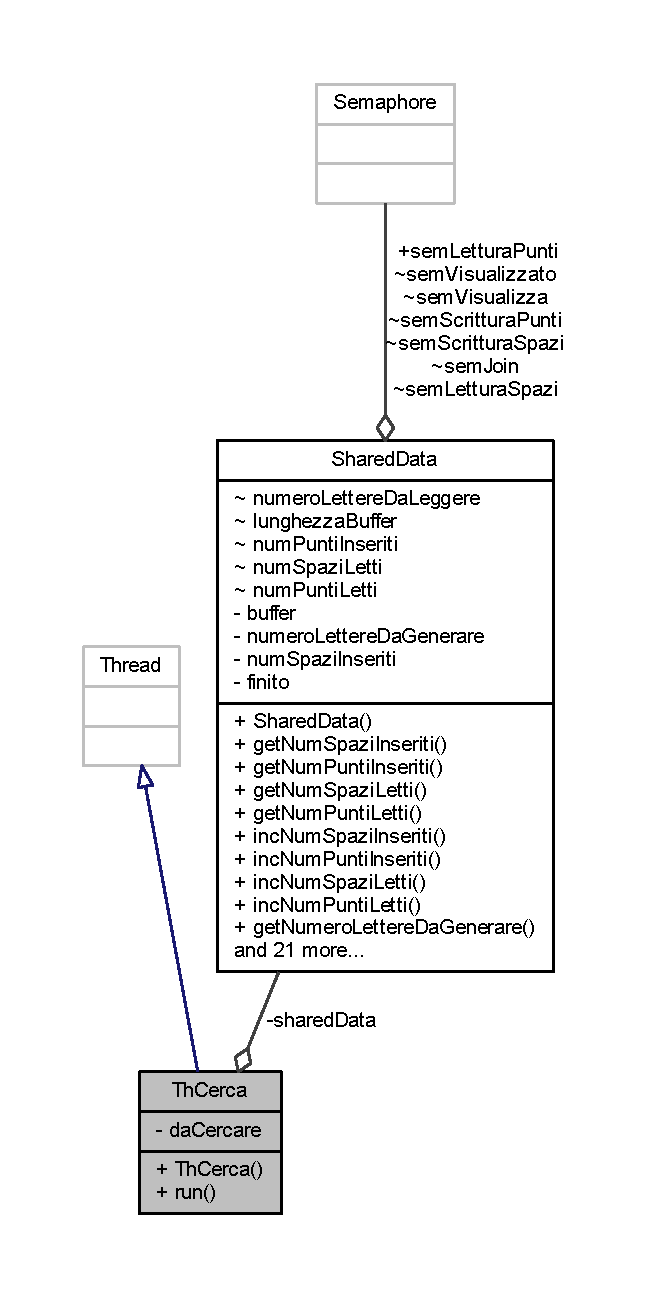
\includegraphics[height=550pt]{classmain_1_1_th_cerca__coll__graph}
\end{center}
\end{figure}
\subsection*{Public Member Functions}
\begin{DoxyCompactItemize}
\item 
\mbox{\hyperlink{classmain_1_1_th_cerca_ae5572ee8b473eb1a52dfcc4c4363d731}{Th\+Cerca}} (\mbox{\hyperlink{classmain_1_1_shared_data}{Shared\+Data}} \mbox{\hyperlink{classmain_1_1_th_cerca_ac5f1128ef8d0ba91a8214e03732e2662}{shared\+Data}}, char \mbox{\hyperlink{classmain_1_1_th_cerca_a05008a7b42b41e8cb77230f70da26619}{da\+Cercare}})
\item 
void \mbox{\hyperlink{classmain_1_1_th_cerca_a13a43e6d814de94978c515cb084873b1}{run}} ()
\end{DoxyCompactItemize}
\subsection*{Private Attributes}
\begin{DoxyCompactItemize}
\item 
final \mbox{\hyperlink{classmain_1_1_shared_data}{Shared\+Data}} \mbox{\hyperlink{classmain_1_1_th_cerca_ac5f1128ef8d0ba91a8214e03732e2662}{shared\+Data}}
\item 
final char \mbox{\hyperlink{classmain_1_1_th_cerca_a05008a7b42b41e8cb77230f70da26619}{da\+Cercare}}
\end{DoxyCompactItemize}


\subsection{Detailed Description}
\begin{DoxyAuthor}{Author}
Luca Mantica 
\end{DoxyAuthor}


Definition at line 15 of file Th\+Cerca.\+java.



\subsection{Constructor \& Destructor Documentation}
\mbox{\Hypertarget{classmain_1_1_th_cerca_ae5572ee8b473eb1a52dfcc4c4363d731}\label{classmain_1_1_th_cerca_ae5572ee8b473eb1a52dfcc4c4363d731}} 
\index{main\+::\+Th\+Cerca@{main\+::\+Th\+Cerca}!Th\+Cerca@{Th\+Cerca}}
\index{Th\+Cerca@{Th\+Cerca}!main\+::\+Th\+Cerca@{main\+::\+Th\+Cerca}}
\subsubsection{\texorpdfstring{Th\+Cerca()}{ThCerca()}}
{\footnotesize\ttfamily \mbox{\hyperlink{classmain_1_1_th_cerca}{Th\+Cerca}} (\begin{DoxyParamCaption}\item[{\mbox{\hyperlink{classmain_1_1_shared_data}{Shared\+Data}}}]{shared\+Data,  }\item[{char}]{da\+Cercare }\end{DoxyParamCaption})}



Definition at line 20 of file Th\+Cerca.\+java.



\subsection{Member Function Documentation}
\mbox{\Hypertarget{classmain_1_1_th_cerca_a13a43e6d814de94978c515cb084873b1}\label{classmain_1_1_th_cerca_a13a43e6d814de94978c515cb084873b1}} 
\index{main\+::\+Th\+Cerca@{main\+::\+Th\+Cerca}!run@{run}}
\index{run@{run}!main\+::\+Th\+Cerca@{main\+::\+Th\+Cerca}}
\subsubsection{\texorpdfstring{run()}{run()}}
{\footnotesize\ttfamily void run (\begin{DoxyParamCaption}{ }\end{DoxyParamCaption})}



Definition at line 26 of file Th\+Cerca.\+java.

Here is the call graph for this function\+:
\nopagebreak
\begin{figure}[H]
\begin{center}
\leavevmode
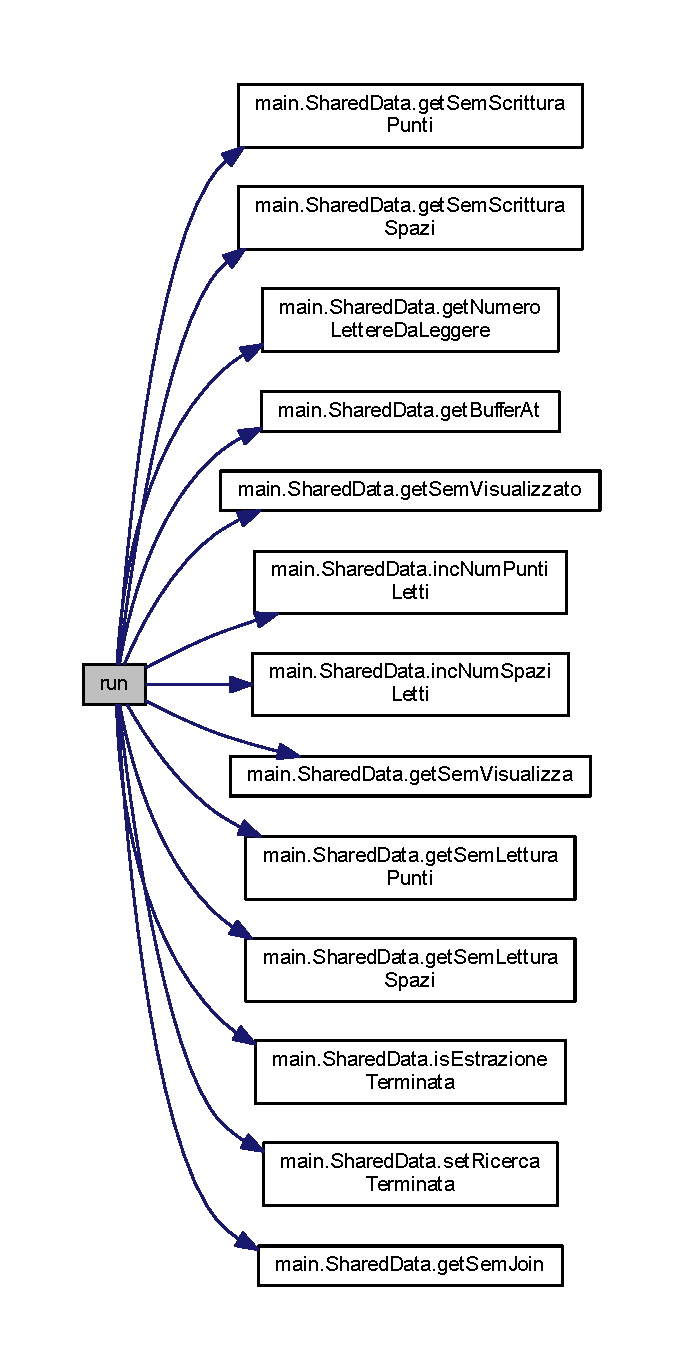
\includegraphics[height=550pt]{classmain_1_1_th_cerca_a13a43e6d814de94978c515cb084873b1_cgraph}
\end{center}
\end{figure}


\subsection{Member Data Documentation}
\mbox{\Hypertarget{classmain_1_1_th_cerca_a05008a7b42b41e8cb77230f70da26619}\label{classmain_1_1_th_cerca_a05008a7b42b41e8cb77230f70da26619}} 
\index{main\+::\+Th\+Cerca@{main\+::\+Th\+Cerca}!da\+Cercare@{da\+Cercare}}
\index{da\+Cercare@{da\+Cercare}!main\+::\+Th\+Cerca@{main\+::\+Th\+Cerca}}
\subsubsection{\texorpdfstring{da\+Cercare}{daCercare}}
{\footnotesize\ttfamily final char da\+Cercare\hspace{0.3cm}{\ttfamily [private]}}



Definition at line 18 of file Th\+Cerca.\+java.

\mbox{\Hypertarget{classmain_1_1_th_cerca_ac5f1128ef8d0ba91a8214e03732e2662}\label{classmain_1_1_th_cerca_ac5f1128ef8d0ba91a8214e03732e2662}} 
\index{main\+::\+Th\+Cerca@{main\+::\+Th\+Cerca}!shared\+Data@{shared\+Data}}
\index{shared\+Data@{shared\+Data}!main\+::\+Th\+Cerca@{main\+::\+Th\+Cerca}}
\subsubsection{\texorpdfstring{shared\+Data}{sharedData}}
{\footnotesize\ttfamily final \mbox{\hyperlink{classmain_1_1_shared_data}{Shared\+Data}} shared\+Data\hspace{0.3cm}{\ttfamily [private]}}



Definition at line 17 of file Th\+Cerca.\+java.



The documentation for this class was generated from the following file\+:\begin{DoxyCompactItemize}
\item 
Statistiche/src/main/\mbox{\hyperlink{_th_cerca_8java}{Th\+Cerca.\+java}}\end{DoxyCompactItemize}

\hypertarget{classmain_1_1_th_gen}{}\section{Th\+Gen Class Reference}
\label{classmain_1_1_th_gen}\index{Th\+Gen@{Th\+Gen}}


Inheritance diagram for Th\+Gen\+:
\nopagebreak
\begin{figure}[H]
\begin{center}
\leavevmode
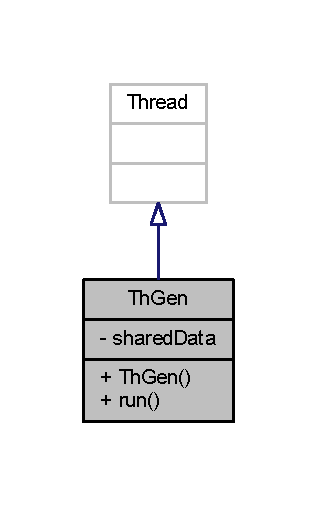
\includegraphics[width=152pt]{classmain_1_1_th_gen__inherit__graph}
\end{center}
\end{figure}


Collaboration diagram for Th\+Gen\+:
\nopagebreak
\begin{figure}[H]
\begin{center}
\leavevmode
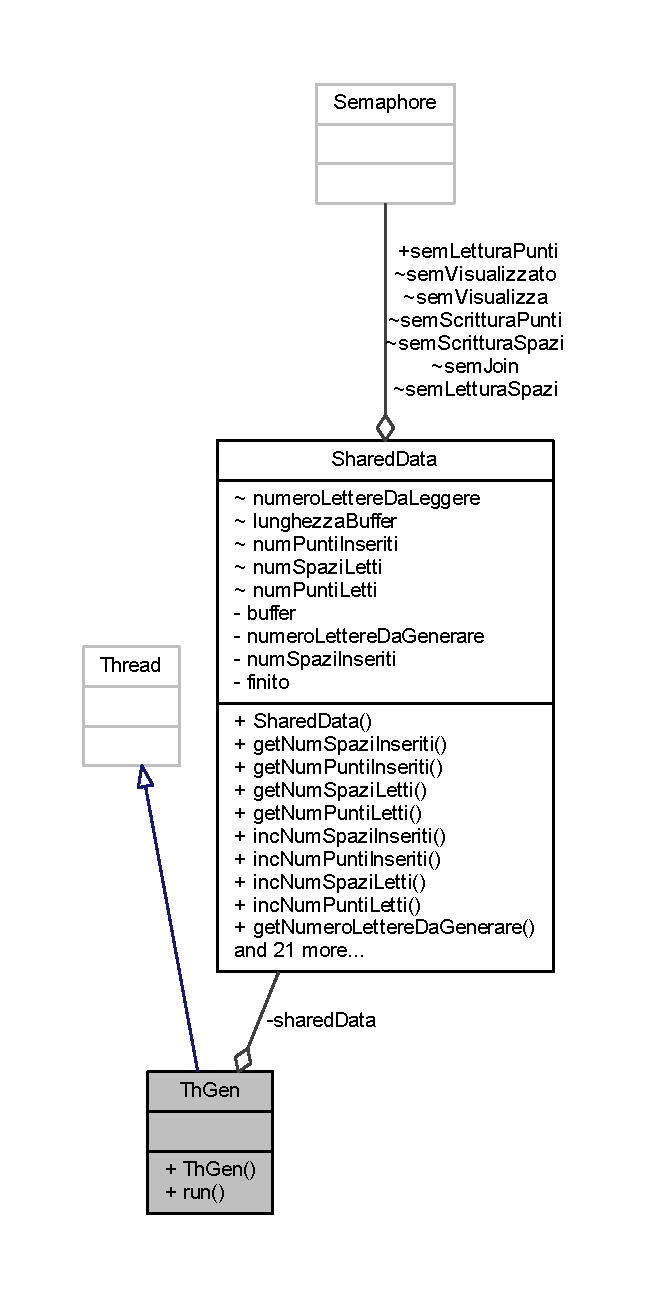
\includegraphics[height=550pt]{classmain_1_1_th_gen__coll__graph}
\end{center}
\end{figure}
\subsection*{Public Member Functions}
\begin{DoxyCompactItemize}
\item 
\mbox{\hyperlink{classmain_1_1_th_gen_ab975ff8819d4ba6b00d6661950d14bb6}{Th\+Gen}} (\mbox{\hyperlink{classmain_1_1_shared_data}{Shared\+Data}} \mbox{\hyperlink{classmain_1_1_th_gen_a1cc1b8edddc4a6929213d3387b370bcd}{shared\+Data}})
\item 
void \mbox{\hyperlink{classmain_1_1_th_gen_a13a43e6d814de94978c515cb084873b1}{run}} ()
\end{DoxyCompactItemize}
\subsection*{Private Attributes}
\begin{DoxyCompactItemize}
\item 
\mbox{\hyperlink{classmain_1_1_shared_data}{Shared\+Data}} \mbox{\hyperlink{classmain_1_1_th_gen_a1cc1b8edddc4a6929213d3387b370bcd}{shared\+Data}}
\end{DoxyCompactItemize}


\subsection{Detailed Description}
\begin{DoxyAuthor}{Author}
mantica\+\_\+luca 
\end{DoxyAuthor}


Definition at line 16 of file Th\+Gen.\+java.



\subsection{Constructor \& Destructor Documentation}
\mbox{\Hypertarget{classmain_1_1_th_gen_ab975ff8819d4ba6b00d6661950d14bb6}\label{classmain_1_1_th_gen_ab975ff8819d4ba6b00d6661950d14bb6}} 
\index{main\+::\+Th\+Gen@{main\+::\+Th\+Gen}!Th\+Gen@{Th\+Gen}}
\index{Th\+Gen@{Th\+Gen}!main\+::\+Th\+Gen@{main\+::\+Th\+Gen}}
\subsubsection{\texorpdfstring{Th\+Gen()}{ThGen()}}
{\footnotesize\ttfamily \mbox{\hyperlink{classmain_1_1_th_gen}{Th\+Gen}} (\begin{DoxyParamCaption}\item[{\mbox{\hyperlink{classmain_1_1_shared_data}{Shared\+Data}}}]{shared\+Data }\end{DoxyParamCaption})}



Definition at line 20 of file Th\+Gen.\+java.



\subsection{Member Function Documentation}
\mbox{\Hypertarget{classmain_1_1_th_gen_a13a43e6d814de94978c515cb084873b1}\label{classmain_1_1_th_gen_a13a43e6d814de94978c515cb084873b1}} 
\index{main\+::\+Th\+Gen@{main\+::\+Th\+Gen}!run@{run}}
\index{run@{run}!main\+::\+Th\+Gen@{main\+::\+Th\+Gen}}
\subsubsection{\texorpdfstring{run()}{run()}}
{\footnotesize\ttfamily void run (\begin{DoxyParamCaption}{ }\end{DoxyParamCaption})}



Definition at line 25 of file Th\+Gen.\+java.

Here is the call graph for this function\+:
\nopagebreak
\begin{figure}[H]
\begin{center}
\leavevmode
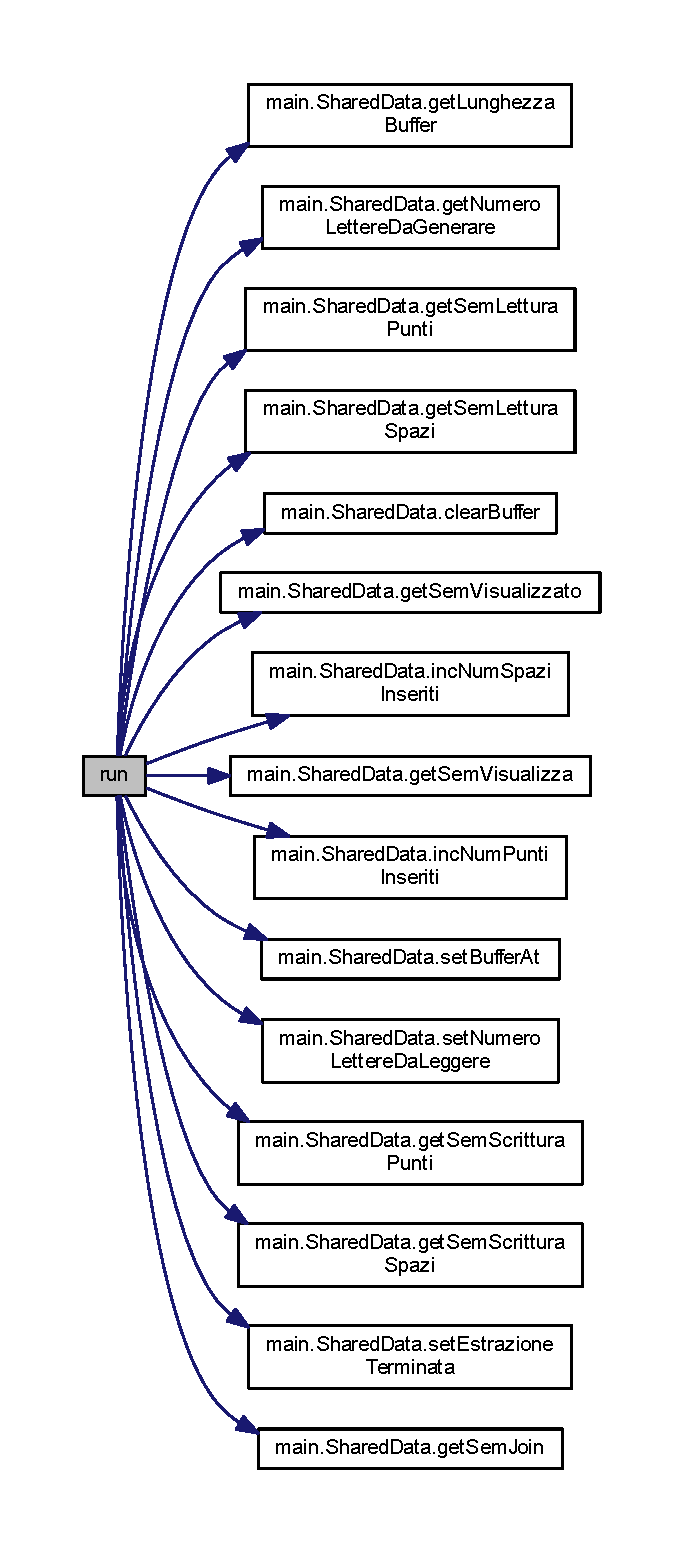
\includegraphics[height=550pt]{classmain_1_1_th_gen_a13a43e6d814de94978c515cb084873b1_cgraph}
\end{center}
\end{figure}


\subsection{Member Data Documentation}
\mbox{\Hypertarget{classmain_1_1_th_gen_a1cc1b8edddc4a6929213d3387b370bcd}\label{classmain_1_1_th_gen_a1cc1b8edddc4a6929213d3387b370bcd}} 
\index{main\+::\+Th\+Gen@{main\+::\+Th\+Gen}!shared\+Data@{shared\+Data}}
\index{shared\+Data@{shared\+Data}!main\+::\+Th\+Gen@{main\+::\+Th\+Gen}}
\subsubsection{\texorpdfstring{shared\+Data}{sharedData}}
{\footnotesize\ttfamily \mbox{\hyperlink{classmain_1_1_shared_data}{Shared\+Data}} shared\+Data\hspace{0.3cm}{\ttfamily [private]}}



Definition at line 18 of file Th\+Gen.\+java.



The documentation for this class was generated from the following file\+:\begin{DoxyCompactItemize}
\item 
Statistiche/src/main/\mbox{\hyperlink{_th_gen_8java}{Th\+Gen.\+java}}\end{DoxyCompactItemize}

\hypertarget{classmain_1_1_th_vis}{}\section{Th\+Vis Class Reference}
\label{classmain_1_1_th_vis}\index{Th\+Vis@{Th\+Vis}}


Inheritance diagram for Th\+Vis\+:
\nopagebreak
\begin{figure}[H]
\begin{center}
\leavevmode
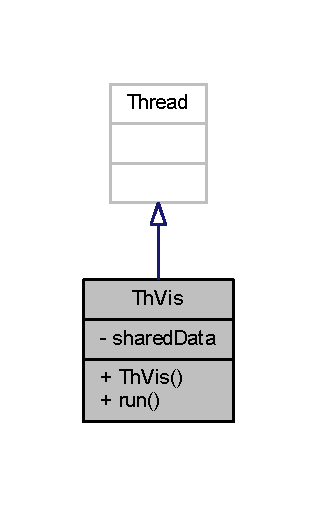
\includegraphics[width=152pt]{classmain_1_1_th_vis__inherit__graph}
\end{center}
\end{figure}


Collaboration diagram for Th\+Vis\+:
\nopagebreak
\begin{figure}[H]
\begin{center}
\leavevmode
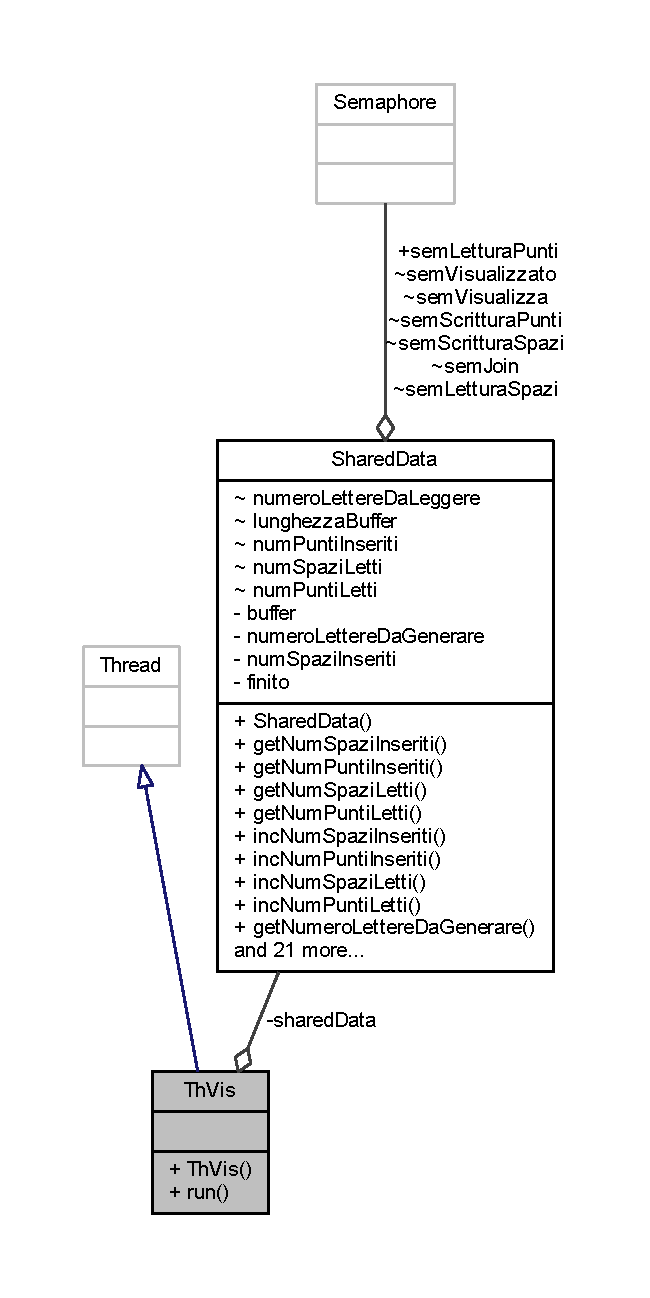
\includegraphics[height=550pt]{classmain_1_1_th_vis__coll__graph}
\end{center}
\end{figure}
\subsection*{Public Member Functions}
\begin{DoxyCompactItemize}
\item 
\mbox{\hyperlink{classmain_1_1_th_vis_aceb31c6e1bd06147c56dfaa16356dc88}{Th\+Vis}} (\mbox{\hyperlink{classmain_1_1_shared_data}{Shared\+Data}} \mbox{\hyperlink{classmain_1_1_th_vis_ac5f1128ef8d0ba91a8214e03732e2662}{shared\+Data}})
\item 
void \mbox{\hyperlink{classmain_1_1_th_vis_a13a43e6d814de94978c515cb084873b1}{run}} ()
\end{DoxyCompactItemize}
\subsection*{Private Attributes}
\begin{DoxyCompactItemize}
\item 
final \mbox{\hyperlink{classmain_1_1_shared_data}{Shared\+Data}} \mbox{\hyperlink{classmain_1_1_th_vis_ac5f1128ef8d0ba91a8214e03732e2662}{shared\+Data}}
\end{DoxyCompactItemize}


\subsection{Detailed Description}
\begin{DoxyAuthor}{Author}
Luca Mantica 
\end{DoxyAuthor}


Definition at line 16 of file Th\+Vis.\+java.



\subsection{Constructor \& Destructor Documentation}
\mbox{\Hypertarget{classmain_1_1_th_vis_aceb31c6e1bd06147c56dfaa16356dc88}\label{classmain_1_1_th_vis_aceb31c6e1bd06147c56dfaa16356dc88}} 
\index{main\+::\+Th\+Vis@{main\+::\+Th\+Vis}!Th\+Vis@{Th\+Vis}}
\index{Th\+Vis@{Th\+Vis}!main\+::\+Th\+Vis@{main\+::\+Th\+Vis}}
\subsubsection{\texorpdfstring{Th\+Vis()}{ThVis()}}
{\footnotesize\ttfamily \mbox{\hyperlink{classmain_1_1_th_vis}{Th\+Vis}} (\begin{DoxyParamCaption}\item[{\mbox{\hyperlink{classmain_1_1_shared_data}{Shared\+Data}}}]{shared\+Data }\end{DoxyParamCaption})}



Definition at line 20 of file Th\+Vis.\+java.



\subsection{Member Function Documentation}
\mbox{\Hypertarget{classmain_1_1_th_vis_a13a43e6d814de94978c515cb084873b1}\label{classmain_1_1_th_vis_a13a43e6d814de94978c515cb084873b1}} 
\index{main\+::\+Th\+Vis@{main\+::\+Th\+Vis}!run@{run}}
\index{run@{run}!main\+::\+Th\+Vis@{main\+::\+Th\+Vis}}
\subsubsection{\texorpdfstring{run()}{run()}}
{\footnotesize\ttfamily void run (\begin{DoxyParamCaption}{ }\end{DoxyParamCaption})}



Definition at line 25 of file Th\+Vis.\+java.

Here is the call graph for this function\+:
\nopagebreak
\begin{figure}[H]
\begin{center}
\leavevmode
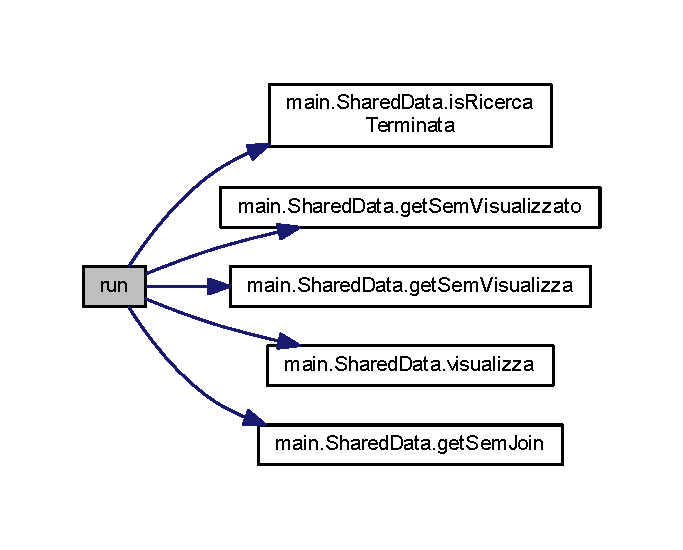
\includegraphics[width=328pt]{classmain_1_1_th_vis_a13a43e6d814de94978c515cb084873b1_cgraph}
\end{center}
\end{figure}


\subsection{Member Data Documentation}
\mbox{\Hypertarget{classmain_1_1_th_vis_ac5f1128ef8d0ba91a8214e03732e2662}\label{classmain_1_1_th_vis_ac5f1128ef8d0ba91a8214e03732e2662}} 
\index{main\+::\+Th\+Vis@{main\+::\+Th\+Vis}!shared\+Data@{shared\+Data}}
\index{shared\+Data@{shared\+Data}!main\+::\+Th\+Vis@{main\+::\+Th\+Vis}}
\subsubsection{\texorpdfstring{shared\+Data}{sharedData}}
{\footnotesize\ttfamily final \mbox{\hyperlink{classmain_1_1_shared_data}{Shared\+Data}} shared\+Data\hspace{0.3cm}{\ttfamily [private]}}



Definition at line 18 of file Th\+Vis.\+java.



The documentation for this class was generated from the following file\+:\begin{DoxyCompactItemize}
\item 
Statistiche/src/main/\mbox{\hyperlink{_th_vis_8java}{Th\+Vis.\+java}}\end{DoxyCompactItemize}

\chapter{File Documentation}
\hypertarget{_main_8java}{}\section{Statistiche/src/main/\+Main.java File Reference}
\label{_main_8java}\index{Statistiche/src/main/\+Main.\+java@{Statistiche/src/main/\+Main.\+java}}
\subsection*{Classes}
\begin{DoxyCompactItemize}
\item 
class \mbox{\hyperlink{classmain_1_1_main}{Main}}
\end{DoxyCompactItemize}
\subsection*{Packages}
\begin{DoxyCompactItemize}
\item 
package \mbox{\hyperlink{namespacemain}{main}}
\end{DoxyCompactItemize}

\hypertarget{_shared_data_8java}{}\section{Statistiche/src/main/\+Shared\+Data.java File Reference}
\label{_shared_data_8java}\index{Statistiche/src/main/\+Shared\+Data.\+java@{Statistiche/src/main/\+Shared\+Data.\+java}}
\subsection*{Classes}
\begin{DoxyCompactItemize}
\item 
class \mbox{\hyperlink{classmain_1_1_shared_data}{Shared\+Data}}
\end{DoxyCompactItemize}
\subsection*{Packages}
\begin{DoxyCompactItemize}
\item 
package \mbox{\hyperlink{namespacemain}{main}}
\end{DoxyCompactItemize}

\hypertarget{_th_cerca_8java}{}\section{Statistiche/src/main/\+Th\+Cerca.java File Reference}
\label{_th_cerca_8java}\index{Statistiche/src/main/\+Th\+Cerca.\+java@{Statistiche/src/main/\+Th\+Cerca.\+java}}
\subsection*{Classes}
\begin{DoxyCompactItemize}
\item 
class \mbox{\hyperlink{classmain_1_1_th_cerca}{Th\+Cerca}}
\end{DoxyCompactItemize}
\subsection*{Packages}
\begin{DoxyCompactItemize}
\item 
package \mbox{\hyperlink{namespacemain}{main}}
\end{DoxyCompactItemize}

\hypertarget{_th_gen_8java}{}\section{Statistiche/src/main/\+Th\+Gen.java File Reference}
\label{_th_gen_8java}\index{Statistiche/src/main/\+Th\+Gen.\+java@{Statistiche/src/main/\+Th\+Gen.\+java}}
\subsection*{Classes}
\begin{DoxyCompactItemize}
\item 
class \mbox{\hyperlink{classmain_1_1_th_gen}{Th\+Gen}}
\end{DoxyCompactItemize}
\subsection*{Packages}
\begin{DoxyCompactItemize}
\item 
package \mbox{\hyperlink{namespacemain}{main}}
\end{DoxyCompactItemize}

\hypertarget{_th_vis_8java}{}\section{Statistiche/src/main/\+Th\+Vis.java File Reference}
\label{_th_vis_8java}\index{Statistiche/src/main/\+Th\+Vis.\+java@{Statistiche/src/main/\+Th\+Vis.\+java}}
\subsection*{Classes}
\begin{DoxyCompactItemize}
\item 
class \mbox{\hyperlink{classmain_1_1_th_vis}{Th\+Vis}}
\end{DoxyCompactItemize}
\subsection*{Packages}
\begin{DoxyCompactItemize}
\item 
package \mbox{\hyperlink{namespacemain}{main}}
\end{DoxyCompactItemize}

%--- End generated contents ---

% Index
\backmatter
\newpage
\phantomsection
\clearemptydoublepage
\addcontentsline{toc}{chapter}{Index}
\printindex

\end{document}
